%
\chapter{Funções a Valores Vetoriais}
%\pagenumbering{arabic}
%
Muitas vezes pensamos em uma curva como uma linha desenhada no papel, como uma reta, um círculo ou uma curva de seno. É útil pensar em uma curva matematicamente como o conjunto de valores de uma função que aplica um intervalo de números reais no plano ou espaço.

Chamaremos tal aplicação de percurso ou caminho. Na maioria das vezes denotamos um caminho por \(\alpha\) ou pelo símbolo $\mathbf{c}$. A imagem do caminho corresponde então a uma reta que vemos no papel (ver Figura~\ref{fig:241}).

Frequentemente, escrevemos \(t\) para a variável independente e imaginamos que seja o tempo, de modo que \(\alpha(t)\) é a posição no tempo \(t\) de uma partícula em movimento, que traça uma curva \(\mathcal{C}\) à medida que \(t\) varia.

\begin{figure}[!ht]
  \centering
  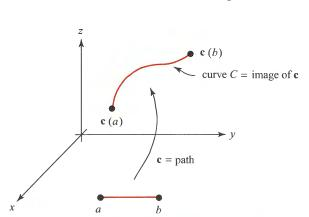
\includegraphics[width=0.6\linewidth]{figura-marsden241.jpg}
  \caption{O percurso é \(\alpha\); a sua imagem é a curva \(\mathcal{C}\)}\label{fig:241}
\end{figure}

Enfatizando estritamente, devemos distinguir entre \(\alpha(t)\) como um ponto no espaço e como um vetor baseado na origem. No entanto, não fazer isso não deve causar confusão. Vejamos algumas ideias,

Diz-se que um vetor \(\alpha\) é a função vetorial
de um argumento escalar \(t\) se cada valor do escalar escolhido
do domínio de valores admissíveis estiver associado a
um valor definido do vetor \(\alpha\). Isso pode ser escrito da seguinte forma,
\begin{equation*}
\alpha= \alpha(t). 
\end{equation*}

Se o vetor \(\alpha\) for uma função do argumento escalar \(t\),
\(\alpha =\alpha(t)\), então as coordenadas \(x\), \(y\), \(z\) do vetor \(r\) também são funções de \(t\) com valores em \(\mathbb{R}\), 
\begin{equation*}
x = x(t),\;  y = y(t),\;  z = z(t). 
\end{equation*}

Por outro lado, se as coordenadas do vetor \(\alpha\) são funções de \(t\), então o próprio vetor \(\alpha\) também é uma função de \(t\),
\begin{equation*}
\alpha = x(t)e_{1} + y(t)e_{2} + z(t)e_{3}. 
\end{equation*}

Portanto, determinar uma função vetorial \(\alpha(t)\) é o mesmo que
determinar três funções escalares ou reais \(x(t)\), \(y(t)\), \(z(t)\).

Um caminho ou percurso em \(\mathbb{R}^{n}\) é uma aplicação \(\alpha \colon [a,\; b] \to  \mathbb{R}^{n}\); é um caminho no plano se \(n=2\) e um caminho no espaço se \(n = 3\). A coleção de pontos \(\alpha(t)\) quando \(t\) varia no intervalo fechado \([a,\; b]\) é chamada de curva, e \(\alpha(a)\) e \(\alpha(b)\) são seus pontos finais. Diz-se que o caminho \(\alpha\) parametriza essa curva.

Se \(\alpha\) é um caminho em \(\mathbb{R}^{3}\), podemos escrever \(\alpha(t) = \langle x(t),\; y (t),\; z (t)\rangle \) e chamar
\(x(t)\), \(y (t)\) e \(z(t)\) de funções componentes de \(\alpha\). Distinguimos as funções de componentes de forma semelhante em \(\mathbb{R}^{2}\) ou, geralmente, em \(\mathbb{R}^{n}\).

\begin{defi}[Hodógrafo]
O hodógrafo da função vetorial \(\alpha(t)\) de um argumento escalar é o lugar geométrico descrito pelo extremo do vetor \(\alpha(t)\), à medida que o escalar 
\(t\) varia, quando a origem do vetor \(\alpha(t)\) é fixada em um ponto \(0\) no espaço. Veja Figura~\ref{fig:1-1}
\end{defi}
\begin{figure}[H]
\centering
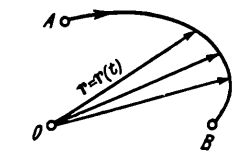
\includegraphics[width=0.5\textwidth]{hodografo-01.jpg}
\caption{Hodógrafo de uma função vetorial \(r=\alpha\)}
\label{fig:1-1}
\end{figure}

O hodógrafo de um raio vetor \(\alpha = \alpha(t)\) de um ponto em movimento é a trajetória \(\mathcal{C}\) desse ponto.
Outra reta \(\mathcal{C}_{1}\)  é o hodógrafo da velocidade \(v = v(t)\) daquele ponto. Veja a Figura~\ref{fig:1-2}
 \begin{figure}[H]
 	\centering
 	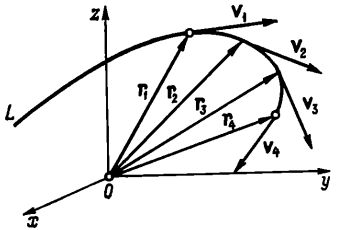
\includegraphics[width=0.5\textwidth]{hodografo-raio-vetor-01.jpg}
 	\caption{Hodógrafo \(\mathcal{C}=L\) de um raio vetor \(\alpha=\alpha(t)=r(t)\)}
 	\label{fig:1-2}
 \end{figure}

Assim, se um ponto material (partícula) está em movimento ao redor de um círculo com velocidade constante, \(\|v\|\; = \; \text{constante}\), então seu hodógrafo de velocidades é igualmente um circunferência com centro em \(0_{1}\) e raio igual a \(\|v\|\). Veja a Figura~\ref{fig:1-3}
 \begin{figure}[H]
	\centering
	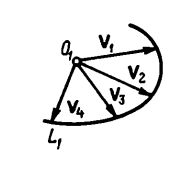
\includegraphics[width=0.5\textwidth]{hodografo-raio-vetor-02.jpg}
	\caption{Hodógrafo \(\mathcal{C}_{1}=L_{1}\) de um raio vetor \(\alpha=\alpha(t)=\text{constante}\)}
	\label{fig:1-3}
\end{figure}



\begin{exc}\label{exem:1-01}
Encontre a função vetorial que descreve 
a linha reta \(\mathcal{L}\) em \(\mathbb{R}^{3}\)  que passa
através do ponto \(P_{0}=(x_{0},\; y_{0},\; z_{0})\) na direção do vetor \(\boldsymbol{\nu}\).
\end{exc}

\solo Trata-se da  imagem do caminho ou percurso
\begin{equation*}
  \alpha(t)=P_{0}+t\,\boldsymbol{\nu}
\end{equation*}
para \(t \in \mathbb{R}\), utilizando ideias de geometria analitica, forma ponto vetor direção. Veja a Figura~\ref{fig:162}). Assim, nossa noção de curva inclui linhas retas como casos especiais. \hfill \(\lozenge\)

\begin{figure}[H]
  \centering
  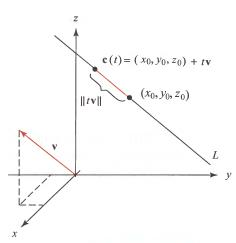
\includegraphics[width=0.45\linewidth]{figura-marsden242.jpg}
  \caption{\(\mathcal{L}\) é a linha reta no espaço através de \(P_{0}\) e na direção \(\boldsymbol{\nu}\); sua equação é
  \(\alpha(t) = P_{0} + t\,\boldsymbol{\nu}.\)}\label{fig:162}
\end{figure}

\begin{exc}\label{exe:1-02}
Encontre a função vetorial da circunferência unitária \(\mathcal{C} \colon x^{2}+y^{2}=1\) no plano \(\mathbb{R}^{2}\).
\end{exc}

\solo
Trata-se a imagem do caminho ou percurso, \(\alpha \colon \mathbb{R} \to \mathbb{R}^{2}\) definido por
\begin{equation*}
\alpha(t) =\langle \cos t, \; \sen t \rangle, \quad 0 \leq t \leq 2\pi
\end{equation*}
(veja a Figura~\ref{fig:243}).

O círculo unitário também é a imagem do caminho \(\widetilde{\alpha}(t) =
\langle \cos 2t,\; \sen 2t\rangle \), \(0 \leq t \leq \pi\). Assim, caminhos diferentes podem parametrizar a mesma curva.
\hfill \(\lozenge\)
\begin{figure}[H]
  \centering
  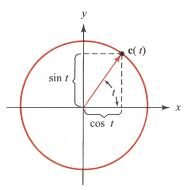
\includegraphics[width=0.3\linewidth]{figura-marsden243.jpg}
  \caption{\(\alpha(t) = \langle\cos t,\; \sen t\rangle\) é um caminho cuja imagem \(\mathcal{C}\) é a circunferência unitária.}\label{fig:243}
\end{figure}


\begin{exc}\label{exe:1-03}
O caminho o percurso \( \alpha(t) =\langle t,\; t^{2}\rangle\) traça um arco parabólico. Esta curva coincide com o gráfico de \(f(x) = x^{2}\). Veja a Figura~\ref{fig:164}.
\end{exc}

\begin{figure}[H]
  \centering
  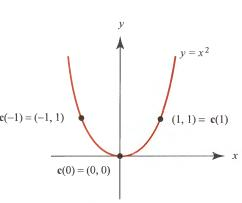
\includegraphics[width=0.4\linewidth]{figura-marsden244.jpg}
  \caption{A imagem de \(\alpha(t) =\langle t,\; t^{2}\rangle \) é a parábola \(y = x^{2}\).}\label{fig:164}
\end{figure}


\begin{exc}
Construa o hodógrafo do vetor \(\alpha=\alpha(t)\) onde 
\begin{equation*}
	\alpha(t) = t\,e_{1}+ t\,e_{2} + t^{2}e_{3}.
\end{equation*}
\end{exc}

\solo
Esta construção pode ser realizada usando pontos e montando uma tabela,
\begin{table}[H]
	\centering
	\begin{tabular}{cccccc}
		\toprule[2pt]
	\(t\)	& 0  & 1 &2  &3  &4  \\
		\midrule
	\(\alpha\)	& 0 & \(\langle 1,\; 1,\; 1 \rangle\) & \(\langle 2,\; 2,\; 4 \rangle\)  & \(\langle 3,\; 3,\; 9 \rangle\) & \(\langle 4,\; 4,\; 16 \rangle\) \\
		\bottomrule[2pt]
	\end{tabular}
\end{table}


Solução alternativa. Denote por \(x\), \(y\), \(z\) as coordenadas do vetor 
\(\alpha\); temos
\begin{equation*}
	x = t,\quad  y = t,\quad  z=t^{2}.
\end{equation*}

Eliminando o parâmetro \(t\) dessas equações, obtemos as equações das superfícies 
\begin{equation*}
	y = x, \quad  z = x^{2}, 
\end{equation*}
cuja reta \(\mathcal{L}\) de intersecção define o hodógrafo do vetor \(\alpha(t)\) Veja a Figura~\ref{fig:1-4}.
\begin{figure}[H]
\centering
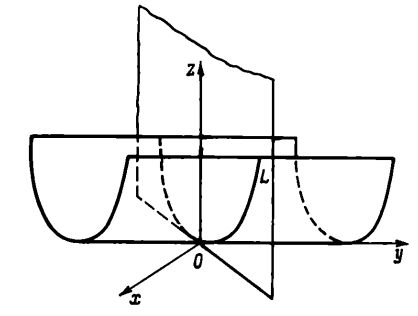
\includegraphics[width=0.5\textwidth]{curve-intersection-two-superficie.jpg}
\caption{Reta \(\mathcal{L}\) de intersecção que define o hodógrafo do vetor}
\label{fig:1-4}
\end{figure}


\begin{exc}\label{exer:5-01}
Seja \(\alpha\) uma função vetorial definida por
\begin{equation*}
\alpha(t)=\sqrt{t-3}\,\boldsymbol{i}+(t-2)^{-1}\, \boldsymbol{j}.
\end{equation*}

Identifique as funções componente e encontre o domínio comum a ambas.
\end{exc}

\solo
(a) As funções componentes \(f(t) = \sqrt{t-3}\) e \(g(t) = (t-2)^{-1}\), são funções reais.

(b) O domínio de \(\alpha\) é o conjunto de valores de \(t\) para os quais as funções \(f\)  e \(g\)
são definidas. O valor da função \(f\) é definido para t \(\geq 3\) e \(g \) é definida para todos os números reais, exceto \(2\).

Portanto, o domínio de \(\alpha\) é dado por conjunto
\begin{equation*}
\{t \; \colon \;  t \geq 3\} \cap \{t \; \colon\;  t \neq 2\}=\{t\; \colon \;  t \geq 3\quad \text{e} \quad  t \neq 2\} = \{t \in \mathbb{R}\colon t \geq 3\}.
\end{equation*}

\begin{exc}\label{exer:5-02}
Seja dada uma função vetorial definida por
\begin{equation*}
  \alpha(t)=2\cos t\,\boldsymbol{i}+ 2\sen t\, \boldsymbol{j}.
\end{equation*}

\rm{(a)} Encontre o domínio da função vetorial;  \rm{(b)} Faça um esboço do gráfico dessa equação;  \rm{(c)} Encontre a equação cartesiana do gráfico.
\end{exc}

\solo
(a) O domínio de \(\alpha\) é o conjunto de todos os números reais. Poderíamos tabular os valores de \(x\) e \(y\) para valores particulares de \(t\).

(b) Calculemos a magnitude ou módulo  do vetor posição, temos para cada \(t\)
\begin{equation*}
\|\alpha(t)\| = \sqrt{4 \cos^{2} t + 4 \sen^{2} t} = 2 \sqrt{\cos^{2} t + \sen^{2} t} = 2.
\end{equation*}

Portanto, o ponto final da representação da posição de cada vetor \(\alpha(t)\) está a duas unidades da origem.

Ao deixar \(t\) assumir todos os números no intervalo fechado \([0,\; 2\pi]\), obtemos uma circunferência com seu centro na origem e raio \(2\). Com isto completamos o gráfico inteiro porque qualquer valor de \(t\) dará um ponto nesta circunferência. Um esboço do círculo é mostrado na Figura~\ref{fig:1541}.

As equações paramétricas do gráfico são
\begin{equation*}
x = 2 \cos t \quad \text{e}\quad  y = 2\sen t
\end{equation*}

(c) Uma equação cartesiana do gráfico pode ser encontrada eliminando o parâmetro \(t\) das duas equações paramétricas, que ao elevar os dois lados de cada equação ao quadrado e adicionar
\begin{equation*}
x^{2} + y^{2} = 4
\end{equation*}

\begin{figure}[H]
  \centering
  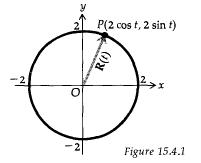
\includegraphics[width=0.4\linewidth]{figura-leithold1541.jpg}
  \caption{Esboço da curva circunferência com \(\alpha(t)=R(t)\)}\label{fig:1541}
\end{figure}


\begin{exc}\label{exer:5-03}
Dadas as equações paramétricas
\begin{equation*}
  x=\cosh t \quad \text{e}\quad y = \senh t
\end{equation*}
\((a)\) Faça um esboço do gráfico dessa equação \((b)\) Encontre a equação cartesiana do gráfico \((c)\) Encontre o domínio
da função vetorial dada.
\end{exc}

\solo
(a) Elevando ao quadrado em ambos os lados das equações dadas e subtraindo, teremos
\begin{equation*}
x^{2}-y^{2} = \cosh^{2} t - \senh^{2} t
\end{equation*}

A partir da identidade \(\cosh^{2} t - \senh^{2} t = 1\), esta equação torna-se
\begin{equation*}
x^{2}-y^{2} = 1
\end{equation*}

A equação resultante é uma equação de uma hipérbole equilátera. Entretanto observe que para todo \(t\) número real,
\(\cosh t\) nunca é menor do que \(1\).

Assim, a curva definida pelas equações paramétricas consiste apenas nos pontos do ramo direito da hipérbole. Um esboço dessa curva é mostrado na Figura~\ref{fig:1543}.

(b) Uma equação cartesiana é
\begin{equation*}
x^{2} - y^{2} = 1, \quad  \text{onde} \quad  x> 1.
\end{equation*}

\begin{figure}[H]
  \centering
  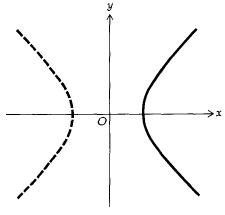
\includegraphics[width=0.4\linewidth]{figura-leithold1543.jpg}
  \caption{Equação Cartesiana do gráfico}\label{fig:1543}
\end{figure}


\bigskip
\noindent\textbf{Observação.}
Conforme afirmado anteriormente, ao eliminar \(t\) das equações paramétricas obtemos uma equação cartesiana. A equação cartesiana resultante, implícita ou explicitamente, define \(y\) como uma ou mais funções dependentes de \(x\).

Ou seja, se \(x = f(t)\) e \(y = g(t)\), então \(y = h(x)\). Se \(h\) é uma função diferenciável de \(x\) e \( f\) é uma função diferenciável de \(t\), segue-se da regra da cadeia usando operadores
\begin{equation*}
D_{t}y = \left(D_{x}y\right)\, \left( D_{t}x\right)
\end{equation*}
ou
\begin{equation*}
g'(t) = (h'(x))\,(f'(t))
\end{equation*}
ou, usando notação diferencial,
\begin{equation*}
\frac{dy}{dt}=\frac{dy}{dx}\,\frac{dx}{dt}
\end{equation*}

Se \(dx/dt \neq 0\), podemos dividir em ambos os lados da equação acima por \(dx/dt\) e obter
\begin{equation}\label{eq:14-3-2}
\frac{dy}{dx}= \dfrac{\dfrac{dy}{dt}}{\dfrac{dx}{dt}}
\end{equation}

A equação \eqref{eq:14-3-2} nos permite encontrar a derivada de \(y\) em relação a \(x\) diretamente a partir das equações paramétricas.

Por outro lado, obtemos a segunda derivada de \(y\) utilizando as equações paramétricas
\begin{equation*}
  \frac{d^{2}y}{dx^{2}}= \frac{d}{dx}\left(\frac{dy}{dx} \right)
\end{equation*}
então
\begin{equation*}
  \frac{d^{2}y}{dx^{2}}=\frac{d}{dx}\left( y'\right)
\end{equation*}

Assim, substituindo a fórmula da primeira derivada, obtemos a fórmula para a segunda derivada,
\begin{equation*}
  \frac{d^{2}\,y}{dx^{2}}= \dfrac{\dfrac{dy'}{dt}}{\dfrac{dx}{dt}}
\end{equation*}

\begin{exc}\label{exer:14-3-3}
Dados as equações paramétricas
\begin{equation*}
x = 3t^{2}\quad \text{e} \quad y = 4t^{3},
\end{equation*}
encontre \(dy/dx\) e \(d^{2}y/dx^{2}\) sem eliminar o parâmetro \( t\).
\end{exc}

\solo
Calculando as derivadas do numerador e denominador da fórmula,
\begin{equation*}
\frac{dy}{dt}= 12t^{2}, \qquad \frac{dx}{dt}=6t \neq 0
\end{equation*}

Substituindo na fórmula deduzida anteriormente,
\begin{equation*}
  \frac{dy}{dx}=\frac{12t^{2}}{6t}=2t.
\end{equation*}

Para calcular a segunda derivada, usando o resultado da primeira derivada \(dy/dx=y'=2t\) e assim,
\begin{equation*}
  \frac{d\, y'}{dt}=\frac{d}{dt}2t=2.
\end{equation*}

Então, novamente substituindo na fórmula,
\begin{equation*}
  \frac{d^{2}}{dx^{2}}=\dfrac{\dfrac{d(y')}{dt}}{\dfrac{dx}{dt}}=\frac{2}{6t}=\frac{1}{3t}, \quad t \neq 0
\end{equation*}


\begin{exc}\label{exer:14-3-4}
Escreva os detalhes da resolução dos itens
\begin{enumerate}
  \item[\rm{(a)}]
Desenhe um esboço do gráfico da curva definida por as equações paramétricas
\begin{equation*}
x = f(t) = 3t^{2} \quad \text{e}\quad y = g(t)=4t^{3}
\end{equation*}
  \item[\rm{(b)}] Encontre uma equação cartesiana do gráfico.
\end{enumerate}
\end{exc}

\solo
Sabemos a forma das equações paramétricas, a saber,
\begin{equation*}
x=f(t)= 3t^{2} \quad \text{e}\quad y = g(t)=4t^{3}
\end{equation*}

\begin{enumerate}
\item[(a)]
Como \(x = 3t^{2}\), concluímos que \(x\) nunca é negativo. Assim o gráfico esta confinado no primeiro e quarto quadrante. A Tabela~\ref{tab:1541}
fornece os valores de \(x\) e\(y\) para valores particulares de \(t\).
\begin{table}[H]
\centering
\begin{tabular}{m{5em} m{5em} m{5em}}
	\toprule[2pt]
\(t\)	& \(x\) & \(y\) \\
	\midrule[1.5pt]
0	& 0 & 0  \\
	\midrule
1/2	& 3/4 & 1/2  \\
	\midrule
1	& 3 & 4 \\
	\midrule
2	& 12 & 32  \\
	\midrule
-1/2	&3/4  & -1/2  \\
	\midrule
-1	&3  & -4 \\
	\midrule
-2	& 12 & -32 \\
	\bottomrule[2.0pt]
\end{tabular}
 \caption{Tabela com valores particulares de \(t\)}\label{tab:1541}
\end{table}

Como \(D_{x}y = 2t\), então que quando \(t = 0\), obtemos \(D_{x}y = 0\); portanto, a reta tangente é horizontal no ponto origem \((0,\; 0)\). Um esboço do gráfico é mostrado na Figura~\ref{fig:1542}.
\begin{figure}[H]
\centering
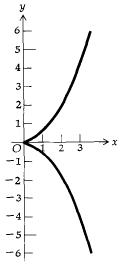
\includegraphics[width=0.2\linewidth]{figura-leithold1542.jpg}
\caption{Esboço do Gráfico das equações Paramétricas}\label{fig:1542}
\end{figure}

\item[(b)]
A partir das duas equações paramétricas \(x = 3t^{2}\) e \(y = 4t^{3}\), obtemos
\begin{equation*}
x^{3} = 27\,t^{6} \quad \text{e} \quad y^{2} = 16\,t^{6}.
\end{equation*}

Resolvendo essa equações para o valor \(t^{6}\) e posteriormente eliminado \( t^{6}\), obtemos,
\begin{equation*}
  \frac{x^{3}}{27}=\frac{y^{2}}{16} \quad \Rightarrow \quad 16\, x^{3} = 27\, y^{2}
\end{equation*}
qual é a equação cartesiana desejada.
\end{enumerate}

O que acontece se derivamos implicitamente a equação cartesiana obtida no item (b)
\begin{equation*}
  48x^{2}=54\,y\,\frac{dy}{dx}\quad \Rightarrow \quad \frac{dy}{dx}=\frac{8x^{2}}{9y}
\end{equation*}

Substituindo \(x\) e \(y\) em termos do parâmetro \(t\) a partir das equações paramétricas fornecidas, obtemos
\begin{equation*}
  \frac{dy}{dx}=\frac{8x^{2}}{9y}=\frac{8(3t^{2})^{2}}{9(4t^{3}}=\frac{72t^{4}}{36t^{3}}=2t
\end{equation*}
o resultado obtido coincide com el valor fornecido pela fórmula de derivação  a 
partir das equações paramétricas, isto é sem conhecer o formato cartesiano da 
função.

%
\section{Cálculo com Funções Vetoriais}
%
Todas as definições de limites, continuidade, derivação e integração indefinida de funções com valores vetoriais envolvem as definições
correspondentes para funções reais do Cálculo Diferencial.

Suponha que uma função vetorial \(\alpha=\alpha(t)\) de um argumento escalar \(t\) 
seja definida em alguma vizinhança do valor \(t_{1}\) do argumento \(t\), exceto 
talvez para o próprio valor \(t_{1}\).

Um vetor constante \(B\) é dito ser o limite do vetor \(\alpha(t)\), quando  
\(t\to t_{1}\), se para qualquer \(\varepsilon > 0\) existe um \(\delta > 0\) tal que para todos os \(t \neq  t_{1}\) que satisfazem a condição \(0< |t-t_{1}|< \delta\) a seguinte desigualdade é verdadeira,
\begin{equation*}
\left|\alpha(t)-B\right| < \varepsilon.
\end{equation*}

Como no caso do cálculo I, escrevemos
\begin{equation*}
 \lim_{t \to t_{1}}\alpha(t)=B.
\end{equation*}

Geometricamente, isso significa que o vetor \(\alpha(t)\) tende, quando \(t\to t_{1}\), ao vetor B tanto em comprimento quanto em direção. Veja a Figura~\ref{fig:1-5}
\begin{figure}[H]
\centering
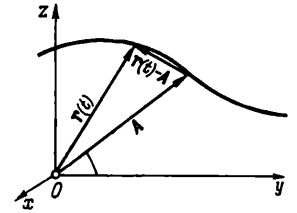
\includegraphics[width=0.5\textwidth]{limite-vetorial.jpg}
\caption{Interpretação geometricamente do limite}
\label{fig:1-5}
\end{figure}

\begin{defi}[Limite em termos de Componentes]\label{def:14-4-1}
Seja \(\alpha\) uma função com valor vetorial, cujos valores de função são dados por
\begin{equation*}
\alpha(t) = f(t)\,e_{1} + g(t)\,e_{2}= f(t)\,\boldsymbol{i} + g(t)\, \boldsymbol{j}.
\end{equation*}

Então, o limite de \(\alpha(t)\) quando \(t\) se aproxima de \(t_{1}\) é definido por
\begin{equation*}
  \lim_{t \to t_{1}}\alpha(t) =\left[\lim_{t \to t_{1}}f(t)\right]e_{1}+ \left[ \lim_{t \to t_{1}}g(t)\right]e_{2}
\end{equation*}
se \(\lim f (t)\) e \(\lim g (t)\) existem quando \( t \to t_{1}\).
\end{defi}

\begin{exc}
  Encontre o limite função vetorial,
  \begin{equation*}
    \alpha(t) = \frac{1-\sqrt{t+1}}{1-t}e_{1} + \frac{t}{t+1}e_{2}\quad \text{ quando} \quad t_{1}=0
  \end{equation*}
\end{exc}

\solo
Como cada função componente possui limite em \(t_{1}\), logo existe o limite da função vetorial, isto,
\begin{equation*}
  \lim_{t \to t_{1}}\frac{1-\sqrt{t+1}}{1-t}=\lim_{t \to 0}\frac{1-\sqrt{t+1}}{1-t}=0
\end{equation*}

Por outro lado calculamos o limite da função racional
\begin{equation*}
\lim_{t \to t_{1}}\frac{t}{t+1}=\lim_{t \to 0}\frac{t}{t+1}=0
\end{equation*}

Finalmente o limite da função vetorial
\begin{equation*}
\lim_{t \to 0}\alpha(t) = \lim_{t \to 0}\frac{1-\sqrt{t+1}}{1-t}\,e_{1} + \lim_{t \to 0}\frac{t}{t+1}\, e_{2}
\end{equation*}
e como cada limite da funções componentes foi calculado temos,
\begin{equation*}
\lim_{t \to 0}\alpha(t) = 0\,e_{1}+0\,e_{2}=(0, \; 0).
\end{equation*}

\begin{defi}[Continuidade]\label{def:14-4-2}
A função de valor vetorial \(\alpha\) é contínua no ponto \(t_{1}\) se e somente se as três condições a seguir forem
satisfeitas;
\begin{tasks}[label=(\alph*),item-indent=4em,label-width=4ex,ref=(\alph*)](2)
\task \(\alpha(t_{1})\) existe;
\task existe \(\lim \alpha(t)\), quando \(t \to t_{1}\);
\task \(\lim \alpha(t) =\alpha(t_{1})\) quando \( t \to t_{1}\).
\end{tasks}
\end{defi}

%
\subsection*{Observação Importante}
%
A partir  Definição~\ref{def:14-4-1} e Definição~\ref{def:14-4-2}, segue-se que a função vetorial \(\alpha\), definida por
\begin{equation*}
\alpha(t) = f(t)\, e_{1} + g(t)\, e_{2},
\end{equation*}
é contínua em \(t_{1}\) se e somente se \(f\) e \(g\) forem contínuas em \(t_{1}\).

Suponha que uma função vetorial \(\alpha = \alpha(t)\) seja definida para todo \(t\) no intervalo \(]a,\; b[\). Tome algum valor \(t \in\; ]a,\; b[\), então dê a \(t\) um incremento \(\Delta t\) tal que \(t+\Delta t \in\; ]a,\; b[\) e encontre o incremento correspondente 
\(\Delta \alpha = \alpha(t + \Delta t) - \alpha(t)\) na função vetorial \(\alpha(t)\). Agora considere a razão 
\begin{equation*}
	\dfrac{\Delta \alpha }{\Delta t}.
\end{equation*}

Se, a razão \(\Delta \alpha/\Delta t\) tem um limite, quando  \(\Delta t\to 0\) então esse limite é chamado de \texttt{derivada} da função vetorial \(\alpha = \alpha(t)\) em relação ao argumento escalar \(t\) para um dado valor \(t\) do argumento e é denotado como \(d\alpha(t)/dt\) ou \(\alpha'(t)\) ou \(\dot{\alpha}(t)\). Assim,
\begin{equation*}
\dfrac{d}{dt}\alpha(t) = \lim_{\Delta t \to 0}\dfrac{\Delta \alpha }{\Delta t}=
\lim_{\Delta t \to 0}\dfrac{\alpha(t+\Delta t)-\alpha(t)}{\Delta t}.
\end{equation*}

Neste caso, a função vetorial \(\alpha=\alpha(t)\) é dita diferenciável.


\begin{defi}[Derivada]\label{def:14-4-3}
Se \(\alpha\) é uma função vetorial, então a derivada de \(\alpha\) é outra função  vetorial, denotada por \(\alpha'\) e definida por
\begin{equation*}
  \alpha'(t)= \lim_{\Delta t\to 0}\frac{\alpha(t+\Delta t) -\alpha(t)}{\Delta t}
\end{equation*}
se esse limite existir.
\end{defi}

Na definição anterior, a expressão
\begin{equation*}
\frac{\alpha(t+\Delta t) -\alpha(t)}{\Delta t}
\end{equation*}
foi usada para representar divisão de um vetor por um escalar que ainda não foi definida. Por esta expressão queremos
dizer
\begin{equation*}
  \frac{1}{\Delta t}\left[\alpha(t+\Delta t) -\alpha(t)\right]
\end{equation*}

A notação com operadores \(D_{t}\alpha(t)\) às vezes é usada no lugar de \(\alpha'(t)\).

Uma interpretação geométrica da Definição~\ref{def:14-4-3} é obtida por considerando representações dos vetores
\(\alpha(t)\), \(\alpha(t + h)\) e \( \alpha'(t)\). Consulte a Figura~\ref{fig:1551}.

\begin{figure}[!h]
  \centering
  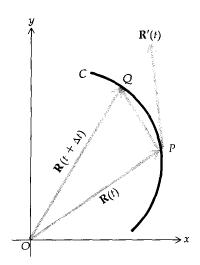
\includegraphics[width=0.3\linewidth]{figura-leithold1551.jpg}
  \caption{Representação Geométrica da derivação de funções Vetoriais}\label{fig:1551}
\end{figure}

A curva \( \mathcal{C}\) é traçada pelo ponto final da representação da posição de \(\alpha(t)\), pois \(t\) assume todos os valores no domínio de \(\alpha\). Seja \(\overrightarrow{OP}\) a representação da posição de \(\alpha(t)\) e \(\overrightarrow{OQ}\) seja a representação da posição de \(\alpha(t+\Delta t)\). Então \(\alpha(t + \Delta t)-\alpha(t)\) é um vetor para o qual \(\overrightarrow{PQ}\) é uma representação. Se o vetor \(\alpha(t + \Delta t)-\alpha(t)\) é multiplicado pelo escalar \(1/\Delta t\), obtemos um vetor com a mesma direção e cuja magnitude é \(1/\Delta t\) vezes a magnitude de \(\alpha(t + \Delta t) - \alpha(t)\).

À medida que \(\Delta t\) se aproxima de zero, o vetor \([\alpha(t + \Delta t)-\alpha(t)]/\Delta t\) se aproxima de um vetor tendo uma de suas representações tangente à curva \( \mathcal{C}\) no ponto \(P\).

O seguinte teorema segue da Definição~\ref{def:14-4-3} e da definição da derivada de uma função real.
\begin{teo}\label{thm:14-4-4}
Se \(\alpha\) é uma função  vetorial definida por
\begin{equation*}
\alpha(t) = f(t)\,e_{1} + g(t)\,e_{2}
\end{equation*}
então
\begin{equation*}
\alpha'(t) = f'(t)\,e_{1} + g'(t)\,e_{2}
\end{equation*}
se \(f'(t)\) e \(g'(t)\) existirem.
\end{teo}

Derivadas de ordem superior de funções com valor vetorial são definidas como derivadas de ordem superior de funções com valor real. Portanto, se \(\alpha\) é uma função de valor vetorial definida por
\begin{equation*}
\alpha(t) = f(t)\,i + g(t)\, j,
\end{equation*}
a segunda derivada de \( \alpha\), denotada por \( \alpha''(t)\), é dada por
\begin{equation*}
\alpha''(t) = D_{t}[\alpha'(t)]
\end{equation*}

Também temos a notação \(D_{t}^{2}\alpha(t)\) no lugar de \(\alpha''(t)\). Aplicando o Teorema~\ref{thm:14-4-4} a \(\alpha'(t)\), obtemos
\begin{equation*}
\mathbf{a}(t)=\alpha''(t) = f''(t)\, i + g''(t)\,j
\end{equation*}
se \(f''(t)\) e \(g''(t)\) existirem.

Se pensarmos em \(\alpha(t)\) como o caminho traçado por uma partícula e como \(t\) é o tempo, é razoável definir o vetor velocidade da seguinte
maneira.

\noindent\textbf{Vetor de Velocidade.}
A velocidade de um caminho \(\alpha\) é definida por
\begin{equation*}
  \alpha'(t)=\lim_{\Delta t \to 0}\frac{\alpha(t+\Delta t)-\alpha(t)}{\Delta t}
\end{equation*}

Normalmente desenhamos o vetor \(\alpha'(t)\) com seu inicio no ponto \(\alpha(t)\). A velocidade do caminho \(\alpha(t)\) é \(s =|\alpha'(t)|\), o comprimento do vetor velocidade. Se \(\alpha(t) = \langle x(t), \; y(t) \rangle\) em \(\mathbb{R}^{2}\), então
\begin{equation*}
\alpha'(t) = \langle x'(t),\; y'(t)\rangle = x'(t)\,i+ y'(t)\,j=x'(t)\,e_{1}+ y'(t)\,e_{2}
\end{equation*}
e se \(\alpha(t) = \langle x(t), \; y (t), \; z'(t)\rangle\) em \(\mathbb{R}^{3}\), então
\begin{equation*}
\alpha'(t) = \langle x'(t),\; y'(t),\; z(t)\rangle= x'(t)\,i+ y'(t)\,j+z'(t)\, k=x'(t)\,e_{1}+ y'(t)\,e_{2}+z'(t)\,e_{3}
\end{equation*}

A teoria dos limites segue a ideia do cálculo de uma variável. Aqui, \(x'(t)\) é a derivada de uma variável comum \(dx/dt\). Se aceitarmos limites de vetores interpretados por componentes, as fórmulas para o vetor velocidade vêm da definição da derivada.

No entanto, o limite também pode ser interpretado no sentido de vetores. Na Figura~\ref{fig:248}, vemos que
\begin{equation*}
\frac{\alpha(t + \Delta t)-\alpha(t)}{\Delta t}\quad  \text{se torna tangente à curva quando}\quad  \Delta t \to 0.
\end{equation*}

\begin{figure}[!h]
  \centering
  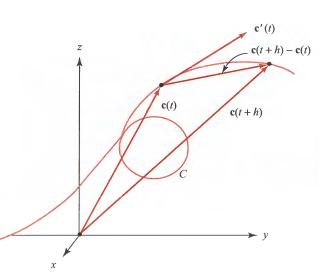
\includegraphics[width=0.5\linewidth]{figura-marsden248.jpg}
  \caption{O vetor \(\alpha'(t)\) é tangente ao caminho \(\alpha(t)\).}\label{fig:248}
\end{figure}

%
\noindent\textbf{Vetor Tangente.}
%
A velocidade \(\alpha'(t)\) é um vetor tangente ao caminho \(\alpha(t)\) no tempo \(t\). Se \(\mathcal{C}\) for uma curva traçada por \(\alpha\) e se \(\alpha'(t)\) não for igual a \(0\), então \(\alpha'(t)\) é um vetor tangente à curva \(\mathcal{C}\) no ponto \(\alpha(t)\).

A velocidade \(\alpha'(t)\) é um vetor tangente ao caminho \(\alpha(t)\). Se pensarmos na derivada \(D\alpha(t)\) como uma matriz, ela será um vetor coluna com as entradas \(x'(t)\), \(y'(t)\) e \(z'(t)\), isto é,
\begin{equation*}
  D\alpha(t)=\left[
  \begin{array}{c}
  x'(t)\\
  y'(t)\\
  z'(t)
  \end{array}
  \right]
\end{equation*}

Lembre-se de que um caminho em $\mathbb{R}^{n}$ é uma função $\alpha$ de $\mathbb{R}$ ou um intervalo $J$ de $\mathbb{R}$ a $\mathbb{R}^{n}$. Se o
caminho é diferenciável, sua derivada em cada instante $t$ é uma matriz $n\times 1$. Especificamente, se $x_{1}(t),\ldots,x_{n}(t)$ são as funções componentes de $\alpha$, a matriz derivada é
\begin{equation*}
\alpha'(t)=\begin{bmatrix}
               \dfrac{d}{dt}x_{1}(t) \\[2ex]
               \dfrac{d}{dt}x_{2}(t)\\[2ex]
               \vdots \\[2ex]
               \dfrac{d}{dt}x_{n}(t)
             \end{bmatrix}
\end{equation*}
que também pode ser escrito em forma de vetor como
\begin{equation*}
\left\langle \frac{d}{dt}x_{1}(t),\; \frac{d}{dt}x_{2}(t), \ldots, \frac{d}{dt}x_{n}(t)\right\rangle \quad \text{ou}\quad \left\langle x'_{1}(t), \; x'_{2}(t), \ldots, x'_{n}(t)\right\rangle.
\end{equation*}

Lembre-se de que $\alpha'(t)$ é o vetor tangente ao percurso no ponto $\alpha(t)$. Lembre-se também de que se $\alpha$ representa o percurso de uma
partícula em movimento, então seu vetor de velocidade é
\begin{equation*}
  v=\alpha'(t)
\end{equation*}
e sua velocidade é $s =\|v\|$. Portanto, a derivada pensada é consistente com nossa noção anterior.

\bigskip
\begin{exc}\label{exer:1-05}
Calcule o vetor tangente ao caminho
\begin{equation*}
\alpha(t) =\langle t,\; t^{2},\; e^{t}\rangle \quad \text{em}  \quad t = 0;
\end{equation*}
\end{exc}

\solo
Derivando uma vez \(\alpha\) obtemos
\begin{equation*}
\alpha'(t) = \langle 1,\; 2t,\; e^{t}\rangle,
\end{equation*}
e assim em \(t=0\) obtemos o vetor tangente representado pela tripla \(\langle 1,\;0,\;1\rangle\).

\begin{exc}\label{exer:1-06}
Descreva o caminho $\alpha(t) = \langle \cos t,\; \sen t,\; t \rangle$. Encontre o vetor de velocidade no ponto da curva imagem onde \(t = \pi/2\).
\end{exc}

\solo Para um dado \(t\), o ponto \((\cos t,\; \sen t,\; 0)\) está no círculo \(x^{2} + y^{2} = 1\) no plano \(xy\). Portanto, o ponto \(\langle \cos t,\; \sen t,\; t\rangle \) encontra-se \(t\) unidades acima do ponto \(\langle \cos t,\; \sen t,\; 0\rangle \) se \(t\) for positivo e \(-t\) unidades abaixo \(\langle \cos t,\; \sen t,\; 0\rangle\) se \(t\) for negativo.

À medida que \(t\) aumenta, \(\langle \cos t,\; \sen t,\; t\rangle \) envolve o cilindro \(x^{2} + y^{2} = 1\) com o aumento da coordenada \(z\).

A curva que isso traça é chamada de \textbf{hélice}, que é representada na Figura~\ref{fig:249}. Em \(t = \pi/2\),
\begin{equation*}
\alpha'(\pi/2) = \left\langle -\sen \frac{\pi}{2}, \cos \frac{\pi}{2},\; 1\right\rangle=\langle-1,\; 0,\; 1\rangle = -i + k.
\end{equation*}

\begin{figure}[H]
  \centering
  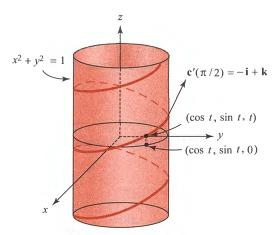
\includegraphics[width=0.5\linewidth]{figura-marsden249.jpg}
  \caption{A hélice \(\alpha(t) = (\cos t,\; \sen t,\; t)\) envolve o cilindro \(x^{2}+y^{2} = 1\).}
  \label{fig:249}
\end{figure}

%
\subsection*{Reta Tangente a um Percurso.}
%
A reta tangente a um caminho em um ponto é a reta que passa pelo ponto na direção do vetor tangente. Usando a forma ponto-direção da equação de uma reta, obtemos a equação paramétrica para a reta tangente.

Se \(\alpha(t)\) é um caminho, sua reta tangente no ponto \(\alpha(t_{0})\) é
\begin{equation*}
l(t) =\alpha(t_{0}) + (t-t_{0})\alpha'(t_{0}).
\end{equation*}

Por conveniência, escrevemos a equação de forma que \(l\) passe por \(\alpha(t_{0})\) em \(t = t_{0}\) (em vez de \(t = 0\)). Veja a Figura~\ref{fig:2411}

\begin{figure}[H]
  \centering
  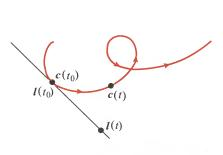
\includegraphics[width=0.5\linewidth]{figura-marsden2411.jpg}
  \caption{A reta tangente a um caminho.}\label{fig:2411}
\end{figure}

\begin{exc}\label{exer:1-07}
Um caminho em \(\mathbb{R}^{3}\) passa pelo ponto \((3,\; 6,\; 5)\) em \(t = 0\) com vetor tangente \(i -j\). Encontre a equação da reta tangente.
\end{exc}

\solo A equação da reta tangente pela definição é
\begin{equation*}
l(t) = (3,\; 6,\; 5) + t(i - j) = (3,\; 6,\; 5) + t (1,\; -1,\; 0) = (3 + t,\; 6 - t,\; 5).
\end{equation*}

Nas coordenadas \((x,\; y,\; z)\), a reta tangente é \(x = 3 + t\), \(y = 6 - t\), \(z = 5\).

Fisicamente, podemos interpretar o movimento ao longo da reta tangente como o caminho que uma partícula em uma curva seguiria se fosse liberada em um determinado momento.

\begin{exc}\label{exer:1-08}
Suponha que uma partícula siga o caminho \(\alpha(t)=\langle e^{t},\; e^{-t},\; \cos t\rangle \) até que voe pela tangente em \(t=1\). Onde se encontra em \(t=3\)?
\end{exc}

\solo Após a derivação de \(\alpha\) obtemos o vetor velocidade,
\begin{equation*}
(e^{t}, \; -e^{-t},\;  -\sen t),
\end{equation*}
que em \(t = 1\) é o vetor \((e,\; -1/e, -\sen 1)\). A partícula está em \((e,\; 1/e,\; \cos 1)\) em \(t=1\).

A equação da reta tangente é
\begin{equation*}
l(t) = \left(e,\; \frac{1}{e}, \cos 1\right) + (t - 1) \left(e,\; -\frac{1}{e},\; -\sen 1\right).
\end{equation*}

Em \(t = 3\), a posição nesta linha é
\begin{equation*}
l(3)=\left(e,\; \dfrac{1}{e},\; \cos 1 \right)+2\left( e,\; \dfrac{1}{e},\; -\sen 1 \right)=\left(3e,\;-\frac{1}{e}, \; \cos 1-2\sen 1  \right)
\end{equation*}
e assim conclui-se o exercício. \hfill $\lozenge$


\begin{exc}
Calcular a segunda derivada das seguintes funções vetoriais,
\begin{align*}
\rm{(a)} & \quad \alpha(t)=(4+\sen t)\, i + \cos t\, j \quad &\rm{(b)}&\quad \beta(t)=\ln t\, i + (1/t) \, j
\end{align*}
\end{exc}

\solo
Derivando as funções vetoriais utilizando as regras de derivação
\begin{enumerate}
  \item[(a)]
  \begin{equation*}
    \alpha'(t)=\cos t\, i -\sen t\, j
  \end{equation*}
  e segunda derivada resulta em
\begin{equation*}
    \alpha''(t)=-\sen t\, i -\cos t\, j
  \end{equation*}

  \item[(b)]
  \begin{equation*}
\beta'(t)=(1/t)\, i - (1/t^{2}) \, j
  \end{equation*}
e a sua segunda derivada,
  \begin{equation*}
\beta''(t)=-(1/t^{2})\, i +(2/t^{3}) \, j
  \end{equation*}
\end{enumerate}


\begin{defi}\label{def:14-5-5}[Derivada num intervalo]
Uma função de valor vetorial \(\alpha\) é dita como diferenciável em um intervalo se \(\alpha'(t)\) existe para todos
os valores de \(t\) no intervalo.
\end{defi}

Os teoremas a seguir fornecem fórmulas de diferenciação para funções com valor vetorial. As provas são baseadas no
Teorema~\ref{thm:14-4-4} e teoremas sobre diferenciação de funções de valor real.
\begin{teo}[Derivada da Soma]\label{thm:14-5-6}
Se \(\alpha\) e \(\beta\) são funções com valor vetorial diferenciável em um intervalo, então \(\alpha + \beta\) é
diferenciável no intervalo, e
\begin{equation*}
D_{t}[\alpha(t) +\beta(t)] = D_{t}\alpha(t) + D_{t}\beta(t)
\end{equation*}
\end{teo}

A prova desse teorema é deixada para o estudante da disciplina.

\begin{exc}
Calcule por separado cada lado da conclusão do Teorema~\ref{thm:14-5-6} para duas funções vetoriais dadas por,
\begin{equation*}
\alpha(t)=t^{2}\, i +(t-2)\,j \quad \text{e} \quad  \beta(t)=\sen t\, i+\cos t\, j.
\end{equation*}
\end{exc}

\solo
Primeiro somando a duas funções vetoriais, componente a componente
\begin{equation*}
  \alpha(t)+\beta(t)=(t^{2}+\sen t)\, i + (t-2+\cos t)\,j
\end{equation*}

Derivando a soma \( \alpha+ \beta\) temos,
\begin{equation*}
D_{t}[\alpha(t)+\beta(t)]=D_{t}[\alpha(t)]\, i +D_{t}[\beta(t)]\, j=(2t+\cos t)\, i +(1-\sen t)\, j
\end{equation*}

Por outro lado derivando separadamente cada função vetorial,
\begin{equation*}
  D_{t}[\alpha(t)]=(2t)\, i + j\quad \text{e}\quad D_{t}[\beta(t)]=\cos t\, i -\sen t\, j
\end{equation*}

Calculando a soma de derivadas,
\begin{equation*}
  D_{t}[\alpha(t)]+D_{t}[\beta(t)] = (2t+\cos t)\, i +(1-\sen t)\, j
\end{equation*}

Assim sendo temos verificado a válido a fórmula da conclusão do Teorema, isto é,
\begin{equation*}
D_{t}[\alpha(t) +\beta(t)] = D_{t}\alpha(t) + D_{t}\beta(t)
\end{equation*}


\begin{teo}\label{thm:14-4-7}
Se \( \alpha\) e \(\beta\) são funções com valor vetorial diferenciável em um intervalo, então \(\alpha \cdot \beta\)
é diferenciável no intervalo, e
\begin{equation*}
D_{t}[\alpha(t) \cdot \beta(t)] = [D_{t}\alpha(t)]\cdot \beta(t) + \alpha(t)\cdot  [D_{t}\beta(t)]
\end{equation*}
\end{teo}

\begin{exc}
Considere as funções vetoriais dadas por,
\(\alpha(t)=t^{2}\, i +(t-2)\,j \) e \(\beta(t)=\sen t\, i+\cos t\, j \). Verificar a validade da conclusão do Teorema~\ref{thm:14-4-7}
\end{exc}

\solo
Se observa que nas hipóteses do teorema existe a operação de produto interno de funções vetoriais. Portanto devemos calcular o produto interno logo derivar, isto é,
\begin{equation*}
\alpha(t) \cdot \beta(t)=(t^{2},\; (t-2))\cdot (\sen t, \;\cos t )=t^{2}\sen t+(t-2)\cos t
\end{equation*}

A seguir derivamos a função real  resultante,
\begin{equation*}
D_{t}[\alpha(t) \cdot \beta(t)]=D_{t}[t^{2}\sen t+(t-2)\cos t]=(t^{2}+1)\cos t +(t+2)\sen t
\end{equation*}

Derivando por separado cada função vetorial, obtemos
\begin{equation*}
D_{t}[\alpha(t)]=2t\,i+j \quad \text{e}\quad D_{t}[\beta(t)]=\cos t\, i -\sen t\, j
\end{equation*}

Logo temos a soma derivadas das funções vetoriais com as funções respectivamente, isto é,
\begin{equation*}
[D_{t}\alpha(t)]\cdot \beta(t)=(2t\, i +j)\cdot(\sen t\, i+ \cos t\, j )=2t\sen t+ \cos t
\end{equation*}
e o segundo produto,
\begin{equation*}
\alpha(t)\cdot  [D_{t}\beta(t)]=[t^{2}\, i +(t-2)\, j]\cdot (\cos t\, i-\sen t\, j)=t^{2}\cos t-(t-2)\sen t
\end{equation*}

Somando os resultados obtido em cada somando,
\begin{equation*}
[D_{t}\alpha(t)]\cdot \beta(t)+\alpha(t)\cdot  [D_{t}\beta(t)]=(t^{2}+1)\cos t + (t+2)\sen t.
\end{equation*}

Assim obtemos a igualdade desejada.

\begin{teo}\label{thm:14-4-8}
Se \(\alpha\) é uma função com valor vetorial diferenciável em um intervalo e \(f\) é uma função com valor real diferenciável no intervalo, então
\begin{equation*}
D_{t}({[f(t)][\alpha(t)]} = [D_{t}f(t)]\alpha(t) + f(t)D_{t}\alpha(t)
\end{equation*}
\end{teo}

A prova é deixada para o estudante da disciplina.

A seguir temos a regra da cadeia para funções vetoriais, sua justificação esta baseada na derivada de uma função vetorial e a regra da cadeia de funções reais.

\begin{teo}[Regra da Cadeia]\label{thm:14-4-9}
Suponha que \(F\) seja uma função vetorial, considere \(h\) uma função real e \(G\), uma função vetorial definida por
\begin{equation*}
  G(t) = F(h(t)).
\end{equation*}
 Se \(\phi = h(t)\) e ambas \( \phi'(t)\) e \(D{\phi}G(t)\) existirem, então \(D_{t}G(t)\) existe e é dada por
 \begin{equation*}
   D_{t}G(t)= [D_{\phi}G(t)]\, \phi'(t)
 \end{equation*}
\end{teo}

\begin{exc}
Seja  \(F\) uma função vetorial e considere uma segunda função \(h\) real, definidas por
\begin{equation*}
  F(\phi)=\phi^{2}\, i + e^{\phi}\, j\quad \text{e}\quad h(t) = \sen t
\end{equation*}
Se \(\phi =h(t)\) e \(G(t)=F(h(t))\). Calcular a derivada \( D_{t}G(t)\).
\end{exc}

\solo
Pelas hipóteses temos \( \phi =\sen t\) a função vetorial \( G(t)=\sen^{2} t\, i + e^{\sen t}\, j\). Calculando a derivada de \( G(t)\) usando a definição, obtemos
\begin{equation}\label{eq:14-9-3}
  D_{t}G(t)=2 \cos t \sen t\, i + e^{\sen t}\cos t\, j
\end{equation}

Resta verificar o resultado anterior usando a regra da cadeia para funções vetoriais, Devemos obter o mesmo resultado como e \eqref{eq:14-9-3}. Tarefa para o estudante da disciplina.

\bigskip
A diferenciação de caminhos ou percursos planos ou tridimensionais é facilitada pelas seguintes regras.

%
\noindent\textbf{Resumo das Regras de Diferenciação.}
%
Sejam $\alpha(t)$ e $\beta(t)$ funções diferenciáveis em $\mathbb{R}^{3}$ e $p(t)$ e $q(t)$ sejam funções escalares diferenciáveis
\begin{table}[!h]
  \centering
\begin{tabularx}{\textwidth} { >{\raggedright\arraybackslash}X | >{\raggedright\arraybackslash} X }
 \hline
Soma &   \(\dfrac{d}{dt}\left[\alpha(t)+\beta(t) \right]=\alpha'(t)+\beta'(t)\) \\[2ex]
 \hline
Multiplicação por escalar &   \(\dfrac{d}{dt}\left[p(t)\beta(t) \right]=p'(t)\beta(t)+p(t)\alpha'(t)\)\\[2ex]
\hline
Produto Ponto & \(\dfrac{d}{dt}\left[\alpha(t)\cdot \beta(t) \right]=\alpha'(t)\cdot \beta(t)+\alpha(t)\cdot \beta'(t) \)\\[2ex]
\hline
Produto Cruz & \(\dfrac{d}{dt}\left[\alpha(t)\times \beta(t) \right]=\alpha'(t)\times \beta(t)+\alpha(t)\times \beta'(t) \)\\[2ex]
\hline
Regra da Cadeia &  \(\dfrac{d}{dt}\left[\alpha\left(q(t)\right)\right]=q'(t)\alpha'(q(t))\)\\[2ex]
\hline
\end{tabularx}
\caption{Resumo de Regras de Derivação}
\label{tab:1-1}
\end{table}

Essas regras se justificam aplicando as regras usuais de diferenciação as funções componentes da função vetorial.

%
\subsection*{Integrais de Funções Vetoriais}
%
Uma função vetorial diferenciável $\psi(t)$ é uma antiderivada de uma função vetorial $\alpha(t)$ em um intervalo $J$ se
\begin{equation*}
\frac{d\, \psi}{dt} = \alpha \quad \text{ em cada ponto de } \quad  J.
\end{equation*}

Se $\psi$ é uma antiderivada de $\alpha$ em $J$, pode-se mostrar, mostrando cada componente por vez, que toda antiderivada de $\alpha$ em $J$ tem a
forma $\psi+C$ para algum vetor constante $C$. O conjunto de todas as antiderivadas de $\alpha$ em $J$ é a integral indefinida de $\alpha$ em $J$.

A integral indefinida de $\alpha$ com respeito a $t$ é o conjunto de todas as antiderivadas de $\alpha$, denotadas por
\begin{equation*}
\int \alpha(t)\, dt.
\end{equation*}

Se $\psi$ for qualquer antiderivada de $\alpha$, então
\begin{equation*}
  \int \alpha(t)\, dt = \psi(t) + C.
\end{equation*}


Agora definimos uma integral indefinida (ou antiderivada) de uma função com valor vetorial.
\begin{defi}[Integral Indefinida]\label{def:14-4-10}
Se \(\psi\) é a função de valor vetorial dada por
\begin{equation*}
\psi(t) = f(t)\, e_{1} + g(t)\,e_{2}
\end{equation*}
então a integral indefinida de \(\psi(t)\) é definida por
\begin{equation}\label{eq:14-4-4}
\int \psi(t)\,dt = e_{1}\int f(t)dt + e_{2}\int g(t)\,dt
\end{equation}
\end{defi}

Esta definição é consistente com a definição de uma integral indefinida de uma função de valor real porque se tomarmos a derivada em ambos os lados de \eqref{eq:14-4-4} em relação a \(t\), temos
\begin{equation*}
D_{t} \int \psi(t)\;dt = e_{1}\,D_{t}\int f(t)dt + e_{2}\, D_{t} \int g(t)dt
\end{equation*}
o que fornece
\begin{equation*}
D_{t}\int \psi(t)\; dt = e_{1}\, f(t) + e_{2}\, g(t)= \psi(t)
\end{equation*}

Para cada uma das integrais indefinidas no lado direito de \eqref{eq:14-4-4}, ocorre uma constante escalar arbitrária. Quando cada um desses escalares
é multiplicado por \(i=e_{1}\) ou \(j=e_{2}\), ocorre um vetor constante arbitrário na soma. Então obtemos
\begin{equation*}
\int \psi(t) dt = \alpha(t) + C,
\end{equation*}
onde \(D_{t}\alpha(t) = \psi(t)\) e \(C\) é um vetor constante arbitrário.

As regras aritméticas usuais do cálculo diferencial para integrais indefinidas se aplicam.

Integrais definidas de funções vetoriais são definidas em termos de componentes.
\begin{defi}[Integral Definida]
Se os componentes de $\alpha(t) = f(t)\,i+g(t)\,j+h(t)\,k$ são integráveis sobre $[a,\; b]$, então $\alpha$ também é, e a \textsf{integral definida}
de $\alpha$ de $a$ para $b$ é
\begin{equation*}
\int_{a}^{b}\alpha(t)\, dt=\left(\int_{a}^{b}f(t)\, dt \right)i+\left(\int_{a}^{b}g(t)\, dt \right)j+\left(\int_{a}^{b}h(t)\, dt \right)k
\end{equation*}
\end{defi}

As regras aritméticas usuais do cálculo diferencial para integrais definidas se aplicam
\begin{exc}
Encontre a função de valor vetorial mais geral cuja derivada é
\begin{equation*}
  \psi(t) = \cos t\, e_{1}+ 5\sen t\, e_{2}
\end{equation*}
\end{exc}

\solo
Se  \(D_{t}\alpha(t)=\psi(t)\), então \(\alpha(t) = \displaystyle{\int \psi(t)\, dt}\), ou seja,
\begin{align*}
\alpha(t)&= i\, \displaystyle{\int \cos t\, dt}-5j\,\displaystyle{ \int \sen t\, dt}\\[2ex]
   &= i(\sen t + C_{1}) - 5j(-\cos t + C_{2})\\[2ex]
   &= \sen t\, i +5 \cos  t\, j + (C_{1}\,i - 5C_{2}\,j)\\[2ex]
   &= \sen t\, i + 5 \cos t\, j + C,
\end{align*}
onde \(C\) é uma constante vetorial. \hfill $\lozenge$

\begin{exc}
Encontre o vetor \(\alpha(t)\) para o qual
\begin{equation*}
D_{t}\alpha(t) = e^{-t}\, i + e^{t}\, j \quad \text{e}\quad \alpha(0) = i + j
\end{equation*}
\end{exc}

\solo
Integrando indefinidamente,
\begin{equation*}
\alpha(t) = i\,\int e^{-t}\, dt + j\,\int e^{t}\, dt
\end{equation*}

Então obtemos
\begin{equation*}
\alpha(t) = i\int e^{-t}\,dt +j \int e^{t}\,dt =i\, (-e^{-t}+C_{1}) + j\,(e^{t} + C_{2})
\end{equation*}

Because \(\alpha(0) = i + j\), temos
\begin{equation*}
i + j = i\,(-1 + C_{1}) + j\,(1 +C_{2})
\end{equation*}

Assim
\begin{equation*}
C_{1}-1 = 1 \quad \text{ e } \quad  C_{2} + 1 = 1
\end{equation*}

Portanto,
\begin{equation*}
C_{1} = 2 \quad \text{ e } \quad  C_{2} = 0
\end{equation*}

Assim sendo
\begin{equation*}
\alpha(t) = (-e^{-t} + 2)\,i + e^{t}\,j
\end{equation*}
é o resultado da integração. \hfill $\lozenge$

\begin{exc}
Calcular a integral definida de uma função vetorial,
\begin{equation*}
\int_{0}^{\pi} \left( \cos t\, i+j-2t\, k \right)\, dt
\end{equation*}
\end{exc}

\solo
Aplicando a definição de integral definida de funções vetoriais,
\begin{align*}
\int_{0}^{\pi} \left( \cos t\, i+j-2t\, k \right)\, dt &= \left(\int_{0}^{\pi} \cos t\, dt\right)i+\left(\int_{0}^{\pi} 1 dt\right)j+
\left(\int_{0}^{\pi} -2t\, dt\right)k  \\[2ex]
&=\sen t\Big|_{0}^{\pi}\, i +t\Big|_{0}^{\pi}-t^{2}\Big|_{0}^{\pi}\\[2ex]
&=[0-0]\,i+[\pi -0]\, j-[\pi^{2}-0^{2}]\, k\\[2ex]
&=\pi\,j-\pi^{2}\,k,
\end{align*}
e isso conclui e exercício. \hfill $\lozenge$

\begin{exc}
Encontrar a função de posição de uma partícula a partir de sua função de velocidade e posição inicial.
A velocidade de uma partícula se movendo no espaço é
\begin{equation*}
\frac{d}{dt}\alpha =(\cos t)\, i-(\sen t)\, j + k.
\end{equation*}

Encontre a posição da partícula em função de $t$ se $\alpha(t)=2\,i+k$ quando $t=0$.
\end{exc}

\solo
Nosso objetivo é resolver o problema de valor inicial que consiste em
\begin{equation*}
\frac{d}{dt}\alpha =(\cos t)\, i-(\sen t)\, j + k, \qquad \alpha(0)= 2\,i+k.
\end{equation*}

Integrar ambos os lados da equação diferencial em relação a $t$ fornece
\begin{equation*}
\alpha(t) = (\sen t)\,i+ (\cos t)\,j +t\,k+ C.
\end{equation*}

Em seguida, usamos a condição inicial para encontrar o valor certo para $C$,
\begin{equation*}
(\sen 0)\,i + (\cos 0)\,j + (0)\, k + C = 2\,i + k = \alpha(0)
\end{equation*}
logo
\begin{equation*}
j+C=2\,i+k \quad \text{implica}\quad C=2\,i-j+k.
\end{equation*}

A posição da partícula em função de $t$ é
\begin{equation*}
\alpha(t) = (\sen t+2)\, i + (\cos t-1)\, j + (t+1)\, k.
\end{equation*}

Para verificar (sempre uma boa ideia), podemos ver a partir desta fórmula que
\begin{align*}
D_{t}\alpha(t) &= (\cos t + 0)\, i + (- \sen t - 0)\, j + (1 + 0)\, k\\[2ex]
&= (\cos t)\, i-(\sen t)\, j + k
\end{align*}
portanto,
\begin{equation*}
\alpha(0) = (\sen 0 + 2)\, i + (\cos 0 - 1)\, j + (0 + 1)\, k = 2\, i + k.
\end{equation*}
e isto conclui o exercício. \hfill $\lozenge$

O seguinte teorema será útil mais adiante para entender novos conceitos e resolver alguns exercícios.

\begin{teo} \label{thm:14-4-11}
Se \(\alpha\) é uma função com valor vetorial diferenciável em um intervalo e \(|\alpha(t)|\) é um vetor diferente de
zero de magnitude constante  para todo \(t\) no intervalo, então os vetores \(\alpha(t)\) e \(D_{t}\alpha(t)\) são
ortogonais, isto é,
\begin{equation*}
  \alpha(t)\; \perp\; D_{t}\alpha(t).
\end{equation*}
\end{teo}

\prova
Pela hipóteses $|\alpha(t)|=k$ é constante, então o seu quadrado $|\alpha(t)|^{2}= \alpha(t)\cdot \alpha(t)=k^{2}$. A derivada a ambos os lados desta
e  portanto, pela regra do produto escalar,
\begin{equation*}
0= \frac{d}{dt}\left[\alpha(t)\cdot\alpha(t) \right]=D_{t}\alpha(t)\cdot \alpha(t)+\alpha(t)\cdot D_{t}\alpha(t)=2\alpha(t)D_{t}\alpha(t);
\end{equation*}
então $\alpha(t)\cdot D_{t}\alpha(t)=0$, ou seja, $D_{t}\alpha(t)$ é perpendicular a $\alpha(t)$. \hfill $\square$

\bigskip
A interpretação geométrica do Teorema~\ref{thm:14-4-11} é evidente. Se o vetor \(\alpha(t)\) tem magnitude constante, então a representação da
posição \(\overrightarrow{OP}\) de \(\alpha(t)\) tem seu ponto terminal \(P\) na circunferência com seu centro na origem e raio \(k\). Portanto, o
gráfico de \(\alpha\) é esta circunferência. Como \(D_{t}\alpha(t)\) e \(\alpha(t)\) são ortogonais, \(\overrightarrow{OP}\) é perpendicular a uma
representação de \(D_{t}\alpha(t)\).

A Figura~\ref{fig:1552} mostra um esboço de um quarto da circunferência, a representação de posição \(\overrightarrow{OP}\) de \(\alpha(t)\) e a
representação \(PB\) de \(D_{t}\alpha(t)\).

\begin{figure}[!h]
  \centering
  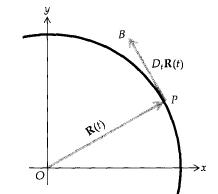
\includegraphics[width=0.4\linewidth]{figura-leithold1552.jpg}
  \caption{Esboço de um parte da Circunferência}\label{fig:1552}
\end{figure}

Para uma curva que descreve um movimento retilíneo uniforme, o vetor velocidade é constante. Em geral, o vetor velocidade é uma função vetorial
$v =\alpha'(t)$ que depende de $t$. A derivada $a=dv/dt =\alpha''(t)$ é chamada de vetor de aceleração da curva. Se a curva for $(x(t),\, y(t),\,
z(t))$, então o vetor de aceleração é
\begin{equation*}
\boxed{\quad \mathbf{a}=x''(t)e_{1}+y''(t)e_{2}+z''(t)e_{3} \quad}
\end{equation*}

\begin{exc}
Uma partícula se move de tal maneira que sua aceleração é constantemente igual a $-e_{3}$. Se a posição quando $t=0$ é $(0,\, 0,\, 1)$ e a
velocidade em $t=0$ é $e_{1}+e_{2}$, quando e onde a partícula cai abaixo do plano $z=0$? Descreva o caminho percorrido pela partícula.
\end{exc}

\solo
Seja $(x(t),\, y(t),\, z(t))$ a curva paramétrica traçada pela partícula, de modo que o vetor velocidade seja
\begin{equation*}
\alpha'(t)=x'(t)e_{1} + y'(t)e_{2}+z'(t)e_{3}.
\end{equation*}

Com a aceleração é  $\alpha''(t)=-e_{3}$, então $x''(t) = 0$, $y''(t) = 0$ e $z''(t)=-1$. Segue-se que $x'(t)$ e $y'(t)$ são funções constantes e
$z'(t)$ é uma função linear com inclinação $-1$.

Como $\alpha'(0)=e_{1}+e_{2}$, obtemos $\alpha'(t)=e_{1}+e_{2}-t\,e_{3}$.

Integrando novamente e usando a posição inicial $(0,\, 0,\, 1)$, encontramos que
\begin{equation*}
(x(t),\; y(t),\; z (t)) = \left(t,\; t,\; 1-(1/2)t^{2}\right).
\end{equation*}

A partícula cai abaixo do plano $z=0$ quando $1-(1/2)t^{2}=0$; ou seja, $t = 2$. Nesse momento, a posição é $\left(\sqrt{2},\, \sqrt{2},\,
0\right)$.

O caminho percorrido pela partícula é uma parábola no plano $y=x$ (ver Figura~\ref{fig:4-1-11-jerrold}) porque neste plano a equação dessa parábola é
descrita por $z=1-(1/2)x^{2}$. \hfill $\lozenge$

\begin{figure}[!h]
  \centering
  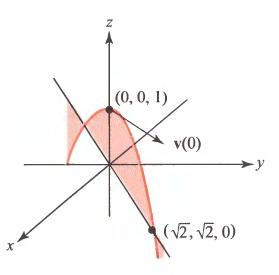
\includegraphics[width=0.45\linewidth]{graphics-4-1-11-jerrold.jpg}
  \caption{O caminho da parábola com posição inicial \((0,\, 0,\, 1)\), velocidade inicial \(e_{1}+e_{2}\) e a aceleração constante \(-e_{3}\) é uma parábola no plano \(y = x\).}
  \label{fig:4-1-11-jerrold}
\end{figure}


A imagem de um caminho $C^{1}$ não é necessariamente ``muito regular''; na verdade, ele pode ter curvas acentuadas ou mudanças de direção.

Por exemplo, o cicloide $\alpha(t) = (t-\sen t,\; 1-\cos t)$ mostrado na Figura~\ref{fig:2-4-6} tem cúspides em todos os pontos onde $\alpha$ toca o
eixo $x$ (isto é, quando $1-\cos t=0$, que acontece quando $t = 2\pi\,n$ com $n = 0, \pm 1, \ldots$).

Outro exemplo é o hipocicloide de nossas cúspides, $\alpha \colon [0,\; 2\pi] \to \mathbb{R}^{2}$, $t \mapsto (\cos^{3} t,\; \sen^{3} t)$, que possui
cúspides em quatro pontos (Figura~\ref{fig:4-1-2-jerrold}).
\begin{figure}[h!]
  \centering
  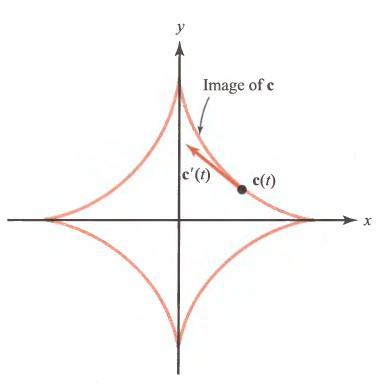
\includegraphics[width=0.45\linewidth]{graphic-4-1-2-jerrold.jpg}
  \caption{A imagem do caminho regular \(\alpha(t) = (\cos 3 t,\; \sen 3 t)\), um hipocicloide, não ``parece regular''.}
  \label{fig:4-1-2-jerrold}
\end{figure}

Em todos esses pontos, entretanto, $\alpha'(t) = 0$, e a reta tangente não está bem definida. Evidentemente, a direção de $\alpha'(t)$ pode mudar
abruptamente em pontos onde ele desacelera para o repouso.

Um caminho diferenciável $\alpha$ é considerado regular em $t=t_{0}$ se $\alpha'(t_{0}) \neq 0$. Se $\alpha'(t) \neq 0$ para todo $t$, dizemos que
$\alpha$ é um caminho regular. Nesse caso, a curva da imagem parece bem regular.

\begin{exc}
Uma partícula se move ao longo de um hipocicloide de acordo com as equações paramétricas,
\begin{equation*}
x = \cos^{3} t, \qquad  y = \sen^{3} t, \quad  a \leq  t \leq  b.
\end{equation*}

Quais são a velocidade e velocidade da partícula?
\end{exc}

\solo
O vetor velocidade da partícula é
\begin{equation*}
 v= \frac{d\, x}{dt}\,i+\frac{d\, y}{dt}\,j=-\left(3\sen t \cos^{2} t\right)\,i + \left(3 \cos t\sen^{2} t\right)\,j,
\end{equation*}
e sua velocidade escalar, o modulo do vetor velocidade, é
\begin{equation*}
s = |v| = \left(9\sen^{2} t \cos^{4} t + 9\cos^{2} t \sen^{4} t\right)^{1/2} = 3|\sen t||\cos t|.
\end{equation*}
e assim conclui-se o exercício. \hfill $\lozenge$

\noindent\textbf{Segunda Lei de Newton.}
Se uma partícula de massa $m$ se move em $\mathbb{R}^{3}$, a força $\mathbf{F}$ agindo sobre ela no ponto $\alpha(t)$ está relacionada à aceleração
pela segunda lei de Newton,
\begin{equation*}
\mathbf{F}(\alpha(t))=m\, \mathbf{a}(t).
\end{equation*}

Em particular, se nenhuma força atuar sobre uma partícula, então $\mathbf{a}(t)=0$, então $\alpha'(t)$ é constante e a partícula segue uma linha
reta.

\noindent\textbf{Aceleração e Segunda Lei de Newton.}
A aceleração de um percurso $\alpha(t)$ é
\begin{equation*}
  \mathbf{a}(t)=\alpha''(t).
\end{equation*}

Se $\mathbf{F}$ é a força atuante e $m$ é a massa da partícula, então
\begin{equation*}
  \mathbf{F}=m\, \mathbf{a}
\end{equation*}

No problema de determinar o caminho $\alpha(t)$ de uma partícula, a lei de Newton torna-se uma equação diferencial (ou seja, uma equação envolvendo
derivadas) para $\alpha(t)$.

\begin{exem}
Um planeta se movendo em torno do Sol (considerado como localizado na origem em $\mathbb{R}^{3}$) ao longo de um caminho $r(t)$ obedece à lei
\begin{equation*}
  m\, \mathbf{r}''=-\frac{G\, m\, M}{r^{3}}\, \mathbf{r}
\end{equation*}
onde $M$ é a massa do sol, $m$ a do planeta, $r = |r|$ e $G$ é a constante gravitacional.
\end{exem}

\solo
A relação usada na determinação da força,
\begin{equation*}
\mathbf{F} = -\frac{G\,m\, M}{r^{3}}\,\mathbf{r},
\end{equation*}
é chamada de lei da gravitação de Newton (ver Figura~\ref{fig:4-1-3-jerrold}).

\begin{figure}[h!]
  \centering
  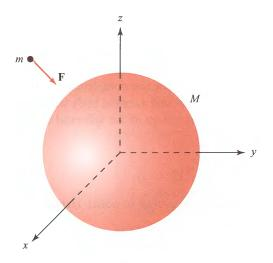
\includegraphics[width=0.45\linewidth]{graphics-4-1-3-Jerrold.jpg}
\caption{Uma massa \(M\) atrai uma massa \(m\) com uma força \(\mathbf{F}\) dada pela lei da gravitação de Newton:
\(\mathbf{F} = -G\,m\,M\, \mathbf{r}/r^{3}\).}
  \label{fig:4-1-3-jerrold}
\end{figure}


Não faremos um estudo geral de tais equações neste texto guia, mas nos contentaremos com o caso especial das órbitas circulares.
(Órbitas mais gerais -as seções cônicas- são discutidas e estudadas num suplemento mais avançado.)

\noindent\textbf{Órbitas Circulares.}
Considere uma partícula de massa $m$ movendo-se a velocidade constante $s$ em um caminho circular de raio $r_{0}$. Supondo que ele se mova no plano
$xy$, podemos suprimir a terceira componente e escrever
\begin{equation*}
\mathbf{r}(t)=\left(r_{0}\cos \dfrac{s\, t}{r_{0}}, \; r_{0}\sen \dfrac{s\,t}{r_{0}}\right),
\end{equation*}
uma vez que este é um círculo de raio $r_{0}$ e $|\mathbf{r}'(t)|=s$. Então
\begin{equation*}
\mathbf{a}(t)=\mathbf{r}''(t)=\left(-\frac{s^{2}}{r_{0}}\cos \frac{s\,t}{r_{0}}, \; -\frac{s^{2}}{r_{0}}\sen \frac{s\,t}{r_{0}} \right)= -\frac{s^{2}}{r_{0}^{2}}\, \mathbf{r}(t).
\end{equation*}

Assim, a aceleração está na direção oposta a $\mathbf{r}(t)$; isto é, ele é direcionado para o centro do círculo (veja a Figura~\ref{fig:4-1-4-jerrold}).

\begin{figure}[h!]
  \centering
  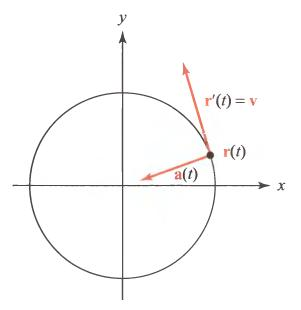
\includegraphics[width=0.35\linewidth]{graphics-4-1-4-jerrold.jpg}
  \caption{A posição, velocidade e aceleração de um partícula em movimento circular.}
  \label{fig:4-1-4-jerrold}
\end{figure}

Essa aceleração multiplicada pela massa da partícula é chamada de \textsf{força centrípeta}. Mesmo que a velocidade escalar é constante, a direção da
velocidade está mudando continuamente, a aceleração é uma taxa de mudança na velocidade escalar ou direção ou em ambas.

A lei de Newton nos ajuda a descobrir uma relação entre o raio da órbita de um corpo giratório e o período, ou seja, o tempo que leva para uma
revolução completa. Considere um satélite de massa $m$ movendo-se com velocidade escalar $s$ em torno de um corpo central de massa $M$ em uma órbita circular de raio $r_{0}$ (distância do centro do corpo central esférico). Pela segunda lei de Newton, $\mathbf{F}= m\, \mathbf{a}$, obtemos
\begin{equation*}
-\frac{s^{2}\, m}{r^{2}_{0}}\, \mathbf{r}(t)= -\dfrac{G\, m\, M}{r_{0}^{3}}\,\mathbf{r}(t).
\end{equation*}

Os comprimentos dos vetores em ambos os lados desta equação devem ser iguais. Por isso
\begin{equation*}
s^{2}= \frac{G\, M}{r_{0}}.
\end{equation*}

Se $T$ denota o período, então $s=2\pi\, r_{0}/T$, substituindo este valor por $s$ na equação acima e resolvendo para $T$, obtemos a seguinte lei,

\noindent\textbf{Lei de Kepler.}
\begin{equation*}
  T^{2}=r_{0}^{3}\,\dfrac{(2\pi)^{2}}{G\, M}.
\end{equation*}

Assim, o quadrado do período é proporcional ao cubo do raio.

Definimos dois conceitos básicos associados a um caminho ou percurso; sua velocidade e sua aceleração. Ambos envolvem cálculo \textsf{diferencial}. O
conceito básico do \textsf{comprimento de um caminho}, que envolve cálculo \textsf{integral}, será abordado na próxima seção.

\begin{exc}
Suponha que um satélite esteja em uma órbita circular em torno da Terra de forma que fique fixo no céu sobre um ponto no equador. Qual é o raio dessa órbita geossíncrona? (A massa da Terra é $5.98 \times 10^{24}$ quilogramas e $G=6.67 \times 10^{-11}$ no sistema de unidades metro-quilograma-segundo.)
\end{exc}

\solo
O período do satélite deve ser de $1$ dia, então $T = 60 \times 60 \times 24 = 86,400$ segundos. Da fórmula
\begin{equation*}
T^{2} = \dfrac{r^{3}_{0}\, (2\pi)^{2}}{G\,M}\quad \text{obtemos}\quad r^{3}_{0} = \dfrac{T^{2}\,G\, M}{(2\pi)^{2}}
\end{equation*}
e assim substituindo os valores dados,
\begin{align*}
r_{0}^{3} &= \frac{T^{2}\, G\, M}{(2\pi)^{2}}= \dfrac{(86,400)^{2}\times (6.67\times 10^{-11})\times (5.98\times 10^{24})}{(2\pi)^{2}}\\[2ex]
      & \approx 7.54 \times 10^{22}\, metros^{3}
\end{align*}

Assim, o raio da órbita é $r_{0} \approx 4.23 \times 10^{7}$ metros $= 42,300$ quilômetros $\approx 26,200$ milhas.


%
\section{Comprimento de Arco}
%
Na disciplina de Cálculo Diferencial obtivemos uma fórmula para encontrar o comprimento do arco de uma curva com uma equação da forma \(y=f(x)\). Este
é um tipo especial de curva porque o gráfico de uma função \(f\) não pode ser cruzado por uma linha vertical em mais de um ponto.

Qual é o comprimento de um percurso $\alpha(t)$? Já que a velocidade escalar $\|\alpha'(t)\|$ é a taxa de variação da distância percorrida em relação ao
tempo, a distância percorrida por um ponto que se move ao longo da curva é a integral da velocidade escalar em relação ao tempo no intervalo
$[t_{0},\; t_{1}]$ do tempo de viagem; ou seja, o comprimento do caminho, também chamado de comprimento do arco, é
\begin{equation*}
\int_{t_{0}}^{t_{1}}\|\alpha'(t)\|\, dt.
\end{equation*}

A seguir desenvolvemos um método para encontrar o comprimento do arco de alguns outros tipos de curvas. Seja \(\mathcal{C}\) a curva com equações
paramétricas
\begin{equation*}
x = f(t) \quad \text{e} \quad   y = g(t)
\end{equation*}
e suponha que \(f\) e \(g\) são contínuas no intervalo fechado \([a,\; b]\).

Desejamos atribuir um número \(L\) para representar o número de unidades para o comprimento do arco de \( \mathcal{C}\) de \(t = a\) a \(t = b\).

Seja \(P\)  uma partição do intervalo fechado \([a,\; b]\) formado pela divisão do intervalo em \(n\) subintervalos escolhendo \(n-1\) números entre \(a\) e \(b\).

Associado a cada número \(t_{i}\) está um ponto \(P_{i}(f(t_{i}),\; g(t_{i}))\) em \( \mathcal{C}\). De cada ponto \(P_{i-1}\) se desenha um segmento
de reta para o próximo ponto \(P_{i}\) (veja a Figura~\ref{fig:1561}).
\begin{figure}[!h]
  \centering
  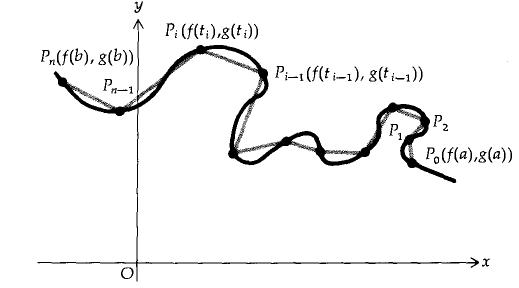
\includegraphics[width=0.6\linewidth]{figura-leithold1561}
  \caption{Noção Geométrica de Comprimento de Arco}\label{fig:1561}
\end{figure}

O número de unidades para comprimento do segmento de reta de \(P_{i-1}\) a \(P_{i}\) é denotado por \(\|\overline{P_{i-1}P_{i}}\|\). Da fórmula da distância temos
\begin{equation*}
\|\overline{P_{i-1}P_{i}}\|=\sqrt{[f(t_{i})-f(t_{i-1})]^{2}+[g(t_{i})-g(t_{i-1})]^{2}}
\end{equation*}

A soma dos números das unidades de comprimento dos $n$ segmentos de linha é
\begin{equation*}
  \sum_{i=1}^{n}\|\overline{P_{i-1}P_{i}}\|
\end{equation*}


\begin{defi}[Comprimento de Arco]\label{def:14-5-1}
	Suponha que a curva \( \mathcal{C}\) tenha equações paramétricas \(x = f (t)\) e \(y = g (t)\). Então, se existe um número \(L\) tendo a propriedade de que para qualquer \(\varepsilon > 0\) existe um \( \delta> 0\) tal que
	\begin{equation*}
		\left|\sum_{i=1}^{n}\|\overline{P_{i-1}P_{i}}\|- L \right| < \varepsilon
	\end{equation*}
	para cada partição \(P\) do intervalo \([a,\; b]\) para a qual a norma \(\|{P}\| <\delta\), escrevemos
	\begin{equation*}
		L=\lim_{|{P}| \to 0}\sum_{i=1}^{n}\|\overline{P_{i-1}P_{i}}\|
	\end{equation*}
	e \(L\) é denominado comprimento do arco da curva \(\mathcal{C}\) do ponto \((f(a),\; g (a))\) ao ponto
	\((f(b),\; g (b))\).
\end{defi}

O arco da curva é \textbf{retificável} se o limite na Definição~\ref{def:14-5-1} existir. Se \(f'\) e \(g'\) são contínuas em \([a,\; b]\), podemos
encontrar uma fórmula para calcular o limite \(L\).

Nossa noção intuitiva do \emph{comprimento do arco} de \(t = a\) até \(t = b\) nos leva a definir o número 
de unidades do comprimento do arco como o limite da soma quando a norma da partição \(|{P}|\) se aproxima de zero.  Uma outra forma mais analítica é a seguinte.

Seja \(\mathcal{C}\) uma curva descrita pela transformação \(\alpha\) de um intervalo fechado 
\([a,\; b]\) em \(\mathbb{R}^{n}\). Considere uma partição \(P =\{t_{i} \in E\vcentcolon i = 0,\ldots, 
k \}\) de \([a, \; b]\) onde \(a = t_{0} < t_{1} <\cdots < t_{k}= b\). Toda partição \(P\) de 
\([a,\; b]\) define uma poligonal  que consiste nos segmentos de reta de \(f(t_{0})\) a \(f(t_{1})\), de \(f(t_{1})\) a \(f(t_{2}),\ldots\), de \(f(t_{k-1})\) a \(f(t_{k})\). (Isso é ilustrado na Figura~\ref{fig:10-1} para o caso \(P=\{t_{0},\; t_{1},\; t_{2},\; t_{3},\; t_{4},\; t_{5}\}\).) Denotamos o  comprimento deste arco poligonal por \(L_{P}\), ou seja,
\begin{equation*}
L_{P} = \sum_{i\,=\, 1}^{n}\|\alpha(t_{i})- \alpha(t_{i-1})\|.
\end{equation*}
\begin{figure}[H]
\centering
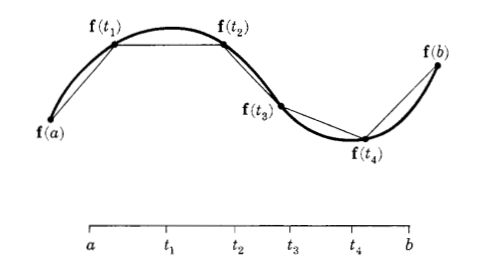
\includegraphics[width=0.5\textwidth]{partition-curve.jpg}
\caption{Um partição \(P\) do intervalo \(E\) com \(\boldsymbol{f}=\alpha\)}
\label{fig:10-1}
\end{figure}

Nossa ideia intuitiva de qual será o comprimento de \(\mathcal{C}\) nos diz que deveríamos ser
capazes de aproximar o comprimento de \(\mathcal{C}\) o máximo que desejarmos medindo os 
comprimentos \(L_{P}\) de arcos poligonais como os descritos. Além disso, como a distância ao 
longo de uma reta deve ser a  menor distância entre pontos, \(L_{P}\) ela deve ser menor que o 
comprimento de \(\mathcal{C}\), e se adicionarmos  pontos à partição \(P\), o comprimento do novo 
arco poligonal deve ser uma aproximação melhor do que  o original para o comprimento do arco 
\(\mathcal{C}\). Isso sugere a seguinte definição. Denotemos por \(\mathcal{P}\) o  conjunto de todas as partições do intervalo \([a,\; b]\).

\begin{defi}[Curva Retificável]
A curva \(\mathcal{C}\) descrita por uma transformação \(\alpha\) de \([a, \; b]\) é dita 
retificável se \(\{L_{P} \vcentcolon P \in \mathcal{P}\}\) tem um limite superior. Se \(\mathcal{C}\) é retificável, o comprimento \(L\) de \(\mathcal{C}\) é o 
supremo de \(\{L_{P} \vcentcolon P \in \mathcal{P}\}\); ou seja,
\begin{equation*}
 L = \sup \{L_{P} \vcentcolon P \in \mathcal{P}\}.
\end{equation*}
\end{defi}	

Este comprimento de uma curva está em conformidade com as ideias intuitivas mencionadas acima. 
Como \(L\) é um limite superior em \(\{L_{P} \vcentcolon P \in \mathcal{P}\}\), \(L\) é maior ou igual ao comprimento \(L_{P}\) de qualquer arco poligonal obtido tomando uma partição \(P\) de \([a,\; 
b]\). Além disso, para qualquer \(\varepsilon > 0\), existe 
uma partição \(P\) de \([a,\;b]\) tal que \(L-\varepsilon < L_{P} \leq  L\); caso contrário, 
\(L\) não seria o supremo (o menor limite superior) de \(\{Lp \vcentcolon P \in \mathcal{P}\}\).
	
Agora mostramos que, se obtivermos uma partição \(P_{2}\) de \([a,\; b]\) adicionando alguns 
pontos à partição \(P_{1}\) de \([a,\;b]\), então \(L_{P_{1}}\leq L_{P_{2}}\). Chamamos \(P_{2}\) 
de \texttt{refinamento} de \(P_{1}\).

\begin{lema}
Se \(P_{2}\) é um refinamento de \(P_{1}\), então 
\begin{equation*}
L_{P_{1}} \leq  L_{P_{2}}.
\end{equation*}
\end{lema}

\prova Este lema é uma consequência simples da desigualdade triangular. Seja \(\tau_{j}\) o primeiro ponto em \(P_{2}\) que não está em \(P_{1}\). Então, para algum \(i\), temos  \(t_{i-1} < \tau_{j} < t_{i}\) e
\begin{align*}
\|\alpha(t_{i})-\alpha(t_{i-1})\|&=\|\alpha(t_{i})-\alpha(\tau_{j}) +\alpha(\tau_{j})-\alpha(t_{i-1})\| \\[2ex]
& \leq \|\alpha(t_{i})-\alpha(\tau_{j})\|+ \|\alpha(\tau_{j})-\alpha(t_{i-1})\|
\end{align*}

Por um número finito de passos, podemos adicionar todos os pontos em \(P_{2}\) a \(P_{1}\) e obter \(L_{P_{1}} \leq  L_{P_{2}}\). \hfill \(\square\)

Se tivéssemos que usar a definição para calcular o comprimento de uma curva, nossa tarefa não 
seria fácil. No entanto, para a maioria das curvas de interesse, podemos encontrar o comprimento 
calculando uma integral.

Consideremos a curva \(\mathcal{C}\) descrita pela transformação \(\alpha\) de \([a,\; b]\) como 
a trajetória de uma partícula, onde $\alpha(t)$ é a posição da partícula no instante \(t\). 
Suponha que \(\alpha\) seja diferenciável em \([a,\; b]\). Então \(\alpha'(t)\) é a velocidade da 
partícula no instante \(t\) e \(|\alpha'(t)|\) é a ``velocidade'' da partícula no instante \(t\). 

Suponhamos que tomemos uma partição \(P\) de \([a,\; b]\) tal que a velocidade ``muda muito 
pouco'' em cada arco de \(f(t_{i-1})\) a \(f(t_{i})\); digamos que seja aproximadamente 
\(\alpha'(t^{\ast})\) neste arco, onde \(t^{\ast} \in [t_{i-1},\; t_{i}]\).

Então, usando a noção elementar de que distância é igual a ``velocidade'' multiplicada pelo 
tempo, o comprimento de \(\mathcal{C}\) é aproximadamente
\begin{equation*}
S_{P}=\sum_{i\,=\, 1}^{k}\|\alpha'(\tau^{\ast})\|(t_{i}-t_{i-1}).
\end{equation*}

Reconhecemos a \(S_{P}\) como a soma aproximada da integral \(\dst \int\|\alpha'(t)\|\,dt\), isto é,
\begin{equation*}
\int_{a}^{b}\|\alpha'(t)\|\,dt=\lim_{|P|\to 0}\, S_{P}
\end{equation*}
onde \(|P|\) denota a norma da partição \(P\),
\begin{equation*}
|P|=\max \{t_{i}-t_{i-1}\vcentcolon i = 1,\ldots, k\},
\end{equation*}
e esse limite significa,

Para \(\varepsilon >0\) existe um \(\delta =\delta(\varepsilon) >0\) tal que se
\begin{equation*}
|P| < \delta \quad \text{implica}\quad \left|S_{P}-\int_{a}^{b}\|\alpha'(t)\|\,dt\right| < \varepsilon
\end{equation*} 

Na discussão anterior, era necessário que a velocidade ``mudasse muito pouco'' no arco. Isso 
significa que precisamos que \(\alpha'\) seja contínua em \([a,\; b]\). Para funções do mundo 
real, sabemos que se uma função \(g\) é contínua em um intervalo fechado, então \(g\) é 
\texttt{uniformemente contínua} em \([a,\; b]\): isto é, para qualquer \(\varepsilon > 0\), 
existe um \(\delta=\delta(\varepsilon) > 0\) tal que
\begin{equation*}
\|g(x)-g(y)\| < \varepsilon\quad  \text{para todo}\quad  x,\; y \in [a,\; b]\quad  \text{sempre que}\quad  |x-y| < \delta.
\end{equation*}

Definimos \texttt{continuidade uniforme} para funções vetoriais da mesma forma e podemos provar 
que, se uma função vetorial é contínua em um intervalo fechado \([a,\; b]\), então ela é uniformemente  contínua  em \([a,\; b]\).

Agora estamos em condições de provar a fórmula integral para o comprimento de uma curva.


\begin{teo}[Curva Retificável]\label{thm:10-4}
Se \(\alpha\) tem uma derivada contínua em \([a,\; b]\), então a curva \(\mathcal{C}\) descrita por \(\alpha\) é retificável e
\begin{equation*}
L(\mathcal{C})=L=\int_{a}^{b}\|\alpha'(t)\|\,dt.
\end{equation*}
\end{teo}

\prova 
Na demonstração, consideramos \(\mathcal{C}\) como uma curva em \(\mathbb{R}^{3}\), embora o 
método possa ser aplicado independentemente da dimensão do espaço em que a curva é definida. Seja 
\(P = \{t_{0},\ldots,t_{k}\}\) uma partição de \([a,\; b]\). Pelo teorema do valor médio, 
\hfill \(\square\)

Formulamos um resultado particular do Teorema~\ref{thm:10-4} que fornece a fórmula do cálculo 
na forma de um teorema em \(\mathbb{R}^{2}\)
\begin{framed}
\begin{teo}\label{thm:15-6-3}
Seja  \( \mathcal{C}\) a curva com equações paramétricas \(x = f(t)\) e \(y = g(t)\), e suponha que \(f'\) e \(g'\)
sejam contínuas no intervalo fechado \([a,\, b]\). Então, o comprimento do arco \(L\)  da curva \(\mathcal{C}\) do
ponto \((f(a),\; g(a))\) ao ponto \((f(b),\; g(b))\) é determinado por
\begin{equation*}
\boxed{\quad  L = L(\mathcal{C})= \int_{a}^{b}\sqrt{[f'(t)]^{2}+[g'(t)]^{2}}\, dt \quad}
\end{equation*}
\end{teo}
\end{framed}


\begin{exc}
Seja \(\mathcal{C}\) a hélice cilíndrica descrita por
\begin{equation*}
\alpha(t) =\langle \cos t,\; \sen t, \; t/2\rangle. 
\end{equation*}
Determine o comprimento \(L\) do arco de \(\mathcal{C}\) de \((1,\; 0,\; 0)\) a 
\((-1,\; 0,\; \pi/2)\).
\end{exc}

\solo
Como \(\alpha(0) = \langle 1,\; 0,\; 0\rangle\) e \(\alpha(\pi) = \langle -1,\; 0,\; 
\pi/2\rangle\), aplicando a fórmula,
\begin{equation*}
L=L(\mathcal{C})=\int_{0}^{\pi}\|\alpha'(t)\|\,dt=\int_{0}^{\pi}\sqrt{\sen^{2}t+\cos^{2} t+1/4}\, dt = \int_{0}^{\pi}\dfrac{\sqrt{5}}{2}\,dt= \dfrac{\sqrt{5}}{2}\,\pi.
\end{equation*} 
 e isso concluí o exercício. \hfill \(\lozenge\) 
 
\begin{exc}
Determine o comprimento da curva \(\mathcal{C}\) descrita por
\begin{equation*}
\alpha(t) =\langle \cos t,\; \sen t \rangle, \quad  t \in [0,\; 4\pi].
\end{equation*}
\end{exc}

\solo 
A curva \(\mathcal{C}\) é o círculo unitário \(C(0,\; 1)\) percorrido duas vezes sob a 
transformação \(\alpha\) de \([0,\; 4\pi]\). Usando o Teorema~\ref{thm:10-4}, obtemos
\begin{equation*}
L=L(\mathcal{C})=\int_{0}^{4\pi}\sqrt{\sen^{2}t+\cos^{2} t}=\int_{0}^{4\pi}\,dt=
4\pi.
\end{equation*}
logo obtemos o resultado desejado. \hfill \(\lozenge\)


\begin{exc}
Encontre o comprimento do arco da curva com equações paramétricas
\begin{equation*}
x = t^{3} \quad \text{e} \quad y = 2\,t^{2},
\end{equation*}
em cada um dos seguintes casos: 
\begin{tasks}[label=(\alph*),item-indent=4em,label-width=4ex,ref=(\alph*)](2)
\task de \(t = 0\) a \(t = 1\);
\task de \(t = -2\) a \(t = 0\).
\end{tasks}
\end{exc}

\solo
Um esboço da curva é mostrado na Figura~\ref{fig:1562}.

\begin{figure}[H]
  \centering
  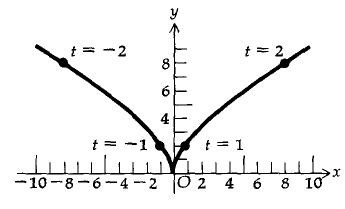
\includegraphics[width=3.0 in]{figura-leithold1562.jpg}
  \caption{Esboço da Curva}\label{fig:1562}
\end{figure}

(a) Fazendo \(x =f(t)\), derivando \(f'(t) = D_{t}x = 3t^{2}\); de forma semelhante \(y = g(t)\), derivando
\(g'(t) = D_{t}y = 4t\).

Portanto, a partir da fórmula dada no Teorema~\ref{thm:15-6-3}, se \(L\)  é o comprimento do arco da curva de \(t = 0\) a \(t = 1\),
\begin{align*}
  L & = \int_{0}^{1}\sqrt{9t^{4}+16t^{2}}\, dt=\int_{0}^{1}\sqrt{t^{2}}\sqrt{9t^{2}+16}\, dt \\[2ex]
    & = \int_{0}^{1}t\,\sqrt{9t^{2}+16}\, dt= \frac{1}{18}\frac{2}{3}\left(9t^{2}+16\right)^{3/2}\Bigg\vert_{t=0}^{1}\\[2ex]
    & =\frac{1}{27}\left[(25)^{3/2}+(16)^{3/2}\right]= \frac{1}{27}\left(125-64\right)=\frac{61}{27}
\end{align*}


(b) Se \(L\)  for o comprimento do arco da curva de \(t = -2\) a \(t = 0\), obtemos novamente usando a fórmula do Teorema~\ref{thm:15-6-3}
\begin{align*}
  L & = \int_{-2}^{0}\sqrt{9t^{4}+16t^{2}}\, dt=\int_{-2}^{0}\sqrt{t^{2}}\sqrt{9t^{2}+16}\, dt \\[2ex]
    & = \int_{-2}^{0}-t\,\sqrt{9t^{2}+16}\, dt=
-\frac{1}{18}\frac{2}{3}\left(9t^{2}+16\right)^{3/2}\Bigg\vert_{t=-2}^{0}\\[2ex]
&=-\frac{1}{27}\left[(16)^{3/2}-(52)^{3/2}\right]= \frac{1}{27}\left(104\sqrt{13}-64\right)\approx 11,5
\end{align*}

Utilizamos no item (a) a propriedade \(\sqrt{t^{2}}=t\) pois \( 0 \leq t \leq 1 \) e no item (b) o fato \( \sqrt{t^{2}}=-t\), pois \( -2 \leq t \leq 0\). \hfill \(\lozenge\)



Para a curva \(\mathcal{C}\) tendo como equações paramétricas \(x=f(t)\) e \(y=g(t)\), seja \(s\)  o comprimento do
arco de \( \mathcal{C}\)  do ponto \((f(t_{0}),\; g (t_{0}))\) ao ponto \((f(t),\; g (t))\), e vamos supor que \(s\)
seja crescente  à medida que \(t\) aumenta. Então \(s=s(t)\) é uma função de \(t\) e é dado por
\begin{equation*}
  s=s(t)=\int_{t_{0}}^{t}\sqrt{[f'(u)]^{2}+[g'(u)]^{2}}\,du
\end{equation*}

Pelo primeiro Teorema fundamental do Cálculo
\begin{equation}\label{eq:4-arc}
  \frac{ds}{dt}=\sqrt{[f'(t)]^{2}+[g'(t)]^{2}}
\end{equation}

A equação vetorial \(\alpha\) da curva \( \mathcal{C}\) e a sua derivada \(\alpha'\) são dadas por
\begin{equation}\label{eq:5-arc}
\alpha(t)=f(t)\, e_{1}+g(t)\, e_{2}\quad \text{e}\quad \alpha'(t)=f'(t)\, e_{1}+g'(t)\, e_{2}
\end{equation}
então o modulo do vetor velocidade é,
\begin{equation}\label{eq:6-arc}
  \|\alpha'(t)\|= \sqrt{[f'(t)]^{2}+[g'(t)]^{2}}.
\end{equation}

Substituindo o resultado dado em \eqref{eq:6-arc} num resultado prévio \eqref{eq:4-arc} obtemos uma nova fórmula
\begin{equation*}
  \boxed{\quad
  \|\alpha'(t)\|=\frac{ds}{dt}. \quad }
\end{equation*}

Da fórmula acima concluímos que se \(s\) for  o comprimento do arco da curva \(\mathcal{C}\) tendo a equação vetorial
\(\alpha\) medido entre algum ponto fixo ao ponto \((f(t),\; g(t))\) onde \(s\) é crescente à medida que \(t\)
aumenta, então a derivada de \(s\) em relação a \(t\) é a magnitude da derivada do vetor posição no ponto \((f(t),\;
g(t))\).

Se substituímos a relação \eqref{eq:6-arc} na fórmula proposta pelo Teorema~\ref{thm:15-6-3}, obtemos
\begin{equation*}
L=L(\mathcal{C}) = \int_{a}^{b} \|\alpha'(t)\|\, dt.
\end{equation*}

Então o Teorema~\ref{thm:15-6-3} pode ter seu formato vetorial proposto no seguinte teorema,

\begin{teo}\label{thm:15-6-4}
Seja a curva \(\mathcal{C}\) com equação vetorial \(\alpha(t) = f(t)\, e_{1} + g (t)\, e_{2}\), e suponha que \(f'\) e \(g'\) sejam contínuos no intervalo fechado \([a,\; b]\). Então, o comprimento do arco de \( \mathcal{C} \), traçado pelo ponto terminal da representação  posicional de \(\alpha(t)\) conforme \(t\) cresce a partir do extremo \(a\) para o extremo \(b\), é determinado por
\begin{equation*}
L = \int_{a}^{b} \|\alpha'(t)\|\, dt.
\end{equation*}
\end{teo}

\prova Tarefa para o leitor. \hfill \(\lozenge\)

\begin{exc}
Encontre o comprimento do arco traçado pelo ponto terminal da representação da posição de \(\alpha(t)\) quando \(t\) cresce de \(t=1\) para \(t=4\) se
\begin{equation*}
\alpha(t) = e^{t} \sen t \, i + e^{t} \cos t \, j
\end{equation*}
\end{exc}

\solo
Calculando o vetor velocidade,
\begin{equation*}
\alpha'(t)= \left(e^{t} \sen t + e^{t} \cos t\right)\, i + \left(e^{t} \cos t -e^{t} \sen t\right)\, j.
\end{equation*}

A seguir calculamos a velocidade escalar,
\begin{align*}
  \|\alpha'(t)\|^{2}&=\left(e^{t} \sen t + e^{t} \cos t\right)^{2} + \left(e^{t} \cos t -e^{t} \sen t\right)^{2}\\[2ex]
  &=e^{2t}\left(\sen^{2} t + 2\sen t \cos t + \cos^{2} t + \cos^{2} t - 2 \sen t \cos t + \sen^{2} t \right)\\[2ex]
  &= 2\,e^{2t}
\end{align*}

Aplicado a fórmula na forma vetorial
\begin{align*}
L&= \int_{1}^{4}\|\alpha'(t)\|\, dt=\int_{1}^{4}\sqrt{ 2\,e^{2t}}\, dt=\int_{1}^{4}\sqrt{2}\,e^{t}\, dt\\[2ex]
&= \sqrt{2}\,e^{t}\Bigg\vert_{t=1}^{4}=\sqrt{2}\,\left(e^{4}-e^{1}\right)=\sqrt{2}\,\left(e^{4}-e\right).
\end{align*}
 e isso concluí o exercício. \hfill \(\lozenge\)


Uma forma alternativa da fórmula dada pelo Teorema~\ref{thm:15-6-3} para o comprimento de um arco de uma curva \(\mathcal{C}\), tendo equações paramétricas \(x = f(t)\) e \(y = g(t)\), é obtida substituindo \(f'(t)\) por \(dx/ dt\) e \(g'(t)\) por \(dy/dt\), ou seja, pelo formato diferencial, o que fornece,
\begin{equation*}
L=\int_{a}^{b}\sqrt{\left( \frac{dx}{dt}\right)^{2}+\left(\frac{dy}{dt}\right)^{2}}\;dt
\end{equation*}


\begin{exc}
Calcular comprimento do arco do caminho
\begin{equation*}
\alpha(t) =\langle r \cos t,\; r \sen t \rangle \quad \text{para} \quad 0 \leq t \leq 2\pi.
\end{equation*}
\end{exc}

\solo
Aplicando a fórmula de comprimento de arco uma vez calculo as derivadas das funções componentes obtemos,
\begin{equation*}
L =\int_{0}^{2\pi}\sqrt{[-r \sen t]^{2} + [r\cos t]^{2}} \, dt = 2\pi r,
\end{equation*}
a circunferência de um círculo de raio \(r\).

Se tivéssemos permitido um domínio de \(0 \leq t \leq 4\pi\), teríamos obtido \(L=4\pi r\), porque o caminho
percorre a mesma circunferência duas vezes (ver Figura~\ref{fig:421})

\begin{figure}[H]
  \centering
  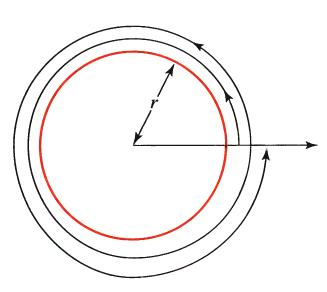
\includegraphics[width=0.3\linewidth]{figura-marsden421.jpg}
  \caption{O comprimento do arco de uma circunferência percorrido duas vezes é \(4\pi r\)}\label{fig:421}
\end{figure}

\bigskip
\noindent\textbf{Comprimento do Arco no Espaço.}
O comprimento da curva (caminho)  \(\alpha(t) =\langle x(t),\; y (t),\; z (t)\rangle \) para \(t_{0} \leq t \leq t_{1}\), é
\begin{equation*}
L=\int_{t_{0}}^{t_{1}}\sqrt{[x'(t)]^{2}+[y'(t)]^{2}+[z'(t)]^{2}}\, dt
\end{equation*}

Para curvas planas, omite-se o termo \(z'(t)\).


\begin{exc}
Encontre o comprimento do arco da curva representada por
 \begin{equation*}
 \alpha(t)=\langle \cos t,\; \sen t,\; t^{2} \rangle,\quad\text{para todo}\quad   0 \leq t  \leq \pi.
 \end{equation*}
\end{exc}

\solo
A função vetorial \(\alpha(t) = \langle \cos t,\; \sen t,\; t^{2}\rangle \) tem o vetor velocidade dado por
\(v =\alpha'(t)= \langle -\sen t, \; \cos t,\;  2t\rangle \). Posto que
\begin{equation*}
  \|\alpha(t)\|=\sqrt{\sen^{2} t+\cos^{2} t+4t^{2}}=\sqrt{1+4t^{2}}=2\sqrt{t^{2}+(1/2)^{2}}
\end{equation*}
o comprimento do arco é
\begin{equation*}
L=\int_{0}^{\pi}2\sqrt{t^{2}+(1/2)^{2}}\, dt.
\end{equation*}

Para calcular a integral usamos a seguinte formula
\begin{equation*}
\int \sqrt{x^{2}+a^{2}}\, dx =\frac{1}{2}\left[x\sqrt{x^{2}+a^{2}}+a^{2}\ln\left(x+\sqrt{x^{2}+a^{2}}  \right) \right]+C
\end{equation*}

Assim
\begin{align*}
  L & = 2\cdot\frac{1}{2}\left[t\sqrt{t^{2}+a^{2}}+(1/2)^{2}\ln \left(t+\sqrt{t^{2}+a^{2}} \right) \right]\Bigg\vert_{t=0}^{\pi} \\[2ex]
   & = \pi \sqrt{\pi^{2}+1/4}+\frac{1}{4}\ln \left(\pi+\sqrt{\pi^{2}+1/4}\right)-\frac{1}{4}\ln\left(\sqrt{{1}/{4}} \right)\\[2ex]
   & = \frac{\pi}{2}\sqrt{1+4\pi^{2}}+\frac{1}{4}\ln\left(2\pi +\sqrt{1+4\pi^{2}}\right) \approx 10,63.
\end{align*}

Para verificar nossa resposta, podemos notar que o caminho \(\alpha\) conecta os pontos \((1,\, 0,\, 0)\) e \((-1,\,
0,\, \pi^{2})\). A distância entre esses pontos é \(\sqrt{4 + \pi^{4}} \approx 10,06\), que é menor que \(10, \, 63\),
como deveria ser.

\bigskip
Se uma curva é composta por um número finito de peças, cada uma das quais \(C^{1}\) (com derivada limitada), calculamos o comprimento do arco adicionando os comprimentos das peças componentes. Essas curvas são chamadas de \(C^{1}\) por partes. Às vezes, apenas dizemos por ``regular por partes''.

\bigskip
\begin{exc}
Uma bola de bilhar em uma mesa quadrada segue o caminho $\alpha \colon [-1,\; 1] \to \mathbb{R}^{3}$ definido por $\alpha(t) =\langle x(t),\; y (t),\; z (t)\rangle =\langle |t|,\; |t-1/2|,\; 0\rangle $. Encontre a distância percorrida pela bola.
\end{exc}

\solo
Este percurso não é regular, porque $x(t) = |t|$ não é diferenciável em $0$, nem é $y(t) = |t-1/2|$ diferenciável em $1/2$. No entanto, se dividirmos o intervalo $[-1,\; 1]$ em partes ou subintervalos,
\begin{equation*}
[-1, \; 0], \quad  [0, \; 1/2], \quad  [1/2, \; 1],
\end{equation*}
vemos que $x(t)$ e $y(t)$ têm derivadas contínuas em cada um dos intervalos $[-1,\; 0]$, $[0,\; 1/2]$ e $[1/2,\; 1]$, (Veja a Figura~\ref{fig:4-2-2-jerrold})

Em $[-1,\; 0]$, $x(t) =-t$, $y(t) =-t + 1/2$ e $z (t) = 0$, então $\|\alpha'(t)\|=\sqrt{2}$. Portanto, o comprimento do arco de $\alpha$ entre $-1$ e
$0$ é dado pela integral definida,
\begin{equation*}
\int_{-1}^{0} \|\alpha'(t)\|\, dt=\int_{-1}^{0} \sqrt{2}\, dt = \sqrt{2}.
\end{equation*}

Da mesma forma, em $[0,\; 1/2]$, $x(t) = t$, $y(t)=-t + 1/2$, $z(t)=0$, e novamente $|\alpha'(t)|=\sqrt{2}$, de modo que o comprimento do arco de
$\alpha$ entre $0$ e $1/2$ é,
\begin{equation*}
\int_{0}^{1/2} \|\alpha'(t)\|\, dt=\int_{0}^{1/2} \sqrt{2}\, dt = \dfrac{1}{2}\sqrt{2}.
\end{equation*}

Finalmente, em $[1/2,\; 1]$ temos $x(t) = t$, $y(t)=t-1/2$, $z(t)=0$, então $|\alpha'(t)|=\sqrt{2}$, de modo que o comprimento do arco de $\alpha$ entre
$1/2$ e $1$ é,
\begin{equation*}
\int_{1/2}^{1} \|\alpha'(t)\|\, dt=\int_{1/2}^{1} \sqrt{2}\, dt = \dfrac{1}{2}\sqrt{2}.
\end{equation*}

Assim, o comprimento total do arco de $\alpha$,
\begin{equation*}
\int_{-1}^{1}\|\alpha'(t)\|\, dt=\int_{-1}^{0}\sqrt{2}\, dt+\int_{0}^{1/2}\sqrt{2}\, dt + \int_{1/2}^{1}\sqrt{2}\, dt =2\sqrt{2},
\end{equation*}
é o resultado que procuramos. \hfill $\lozenge$

\begin{figure}[H]
  \centering
  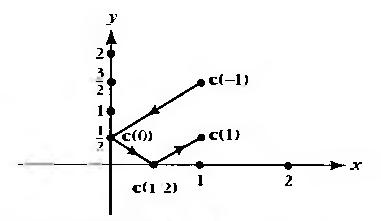
\includegraphics[width=0.6\linewidth]{graphics-4-2-2-jerrold.jpg}
  \caption{Percurso regular por partes}
  \label{fig:4-2-2-jerrold}
\end{figure}

\bigskip
\begin{exc}
Considere o ponto com função de posição
\begin{equation*}
\alpha(t) =\langle t-\sen t,\; 1-\cos t \rangle,
\end{equation*}
que traça o cicloide (veja a Figura~\ref{fig:2-4-6}). Encontre o vetor velocidade, a velocidade escalar e o comprimento de um arco.
\end{exc}

\solo
O vetor velocidade é \(\alpha'(t) =\langle 1- \cos t,\; \sen t\rangle \), então a velocidade escalar do ponto \(\alpha(t)\) é
\begin{equation*}
\|\alpha'(t)\| = \sqrt{(1-\cos t)^{2} + \sen^{2} t} = \sqrt{2 - 2 \cos t}.
\end{equation*}

Consequentemente, \(\alpha(t)\) se move a uma velocidade variável, embora o círculo role a uma velocidade constante.
Além disso, a velocidade de \(\alpha(t)\) é zero quando \(t\) é um múltiplo inteiro de \(2\pi\). Com esses valores de
\(t\), a coordenada \(y\) do ponto \(\alpha(t)\) é zero e, portanto, o ponto está no eixo \(x\). O comprimento do
arco de um ciclo é
\begin{align*}
  L& =\int_{0}^{2\pi}\sqrt{2-2\cos t}\,dt=2\int_{0}^{2\pi}\sqrt{\frac{1-\cos t}{2}}\, dt \\[2ex]
   &= 2\int_{0}^{2\pi}\sen \frac{t}{2}\; dt=4\left(-\cos \frac{t}{2}\right)\Bigg\vert_{t=0}^{2\pi}=8
\end{align*}

Utilizamos a seguintes identidades trigonométricas
\begin{equation*}
1-\cos t=2\sen^{2} \frac{t}{2}\quad \text{e} \quad  \sen \frac{t}{2} \geq 0 \quad  \text{sobre}\quad [0,\; 2\pi]
\end{equation*}

\begin{figure}[H]
  \centering
  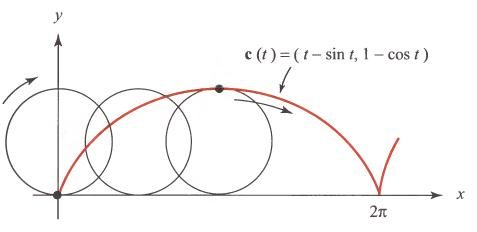
\includegraphics[width=0.6\linewidth]{figura-marsden246.jpg}
  \caption{A curva traçada por um ponto que se move na borda de um círculo rolante é chamada de cicloide.}
  \label{fig:2-4-6}
\end{figure}

\bigskip
\noindent\textbf{O Diferencial do Comprimento do Arco.}
A fórmula do comprimento do arco sugere que se introduza a seguinte notação, que será útil em nossa discussão sobre integrais de linha.

Um \emph{deslocamento infinitesimal} de uma partícula seguindo um caminho
\begin{equation*}
\alpha(t) = x(t)\,e_{1} + y(t)\,e_{2} + z(t)\, e_{3}
\end{equation*}
é
\begin{equation*}
ds=dx\,e_{1}+dy\,e_{2}+dz\,e_{3}=\left(\frac{dx}{dt}e_{1}+\frac{dy}{dt}e_{2}+\frac{dz}{dt}e_{3} \right)\,dt
\end{equation*}
e seu comprimento
\begin{equation*}
\|ds\|=\sqrt{dx^{2}+dy^{2}+dz^{2}}=\sqrt{\left( \frac{dx}{dt}\right)^{2}+\left(\frac{dy}{dt}
\right)^{2}+\left(\frac{dz}{dt} \right)^{2}}\,dt
\end{equation*}
é o diferencial do comprimento do arco. Veja a Figura~\ref{fig:4-2-3}.

\begin{figure}[H]
  \centering
  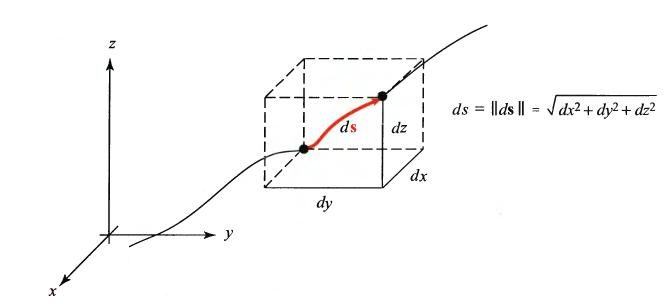
\includegraphics[width=0.7\linewidth]{figura-marsden423.jpg}
  \caption{Diferencial do comprimento do arco.}\label{fig:4-2-3}
\end{figure}

Essas fórmulas nos ajudam a lembrar a fórmula do comprimento do arco como
\begin{equation*}
\boxed{\quad   \text{comprimento do arco}\; = \; \int_{t_{0}}^{t_{1}}\,\|ds\|. \quad}
\end{equation*}

Como fizemos antes com conceitos geométricos como comprimento e ângulo, podemos estender a noção de comprimento do arco para funções vetoriais no espaço \(n\)-dimensional.

\bigskip
\noindent\textbf{Comprimento de Arco n-dimensional.}
Considere \(\alpha\colon [t_{0},\; t_{1}] \to \mathbb{R}^{n}\) uma função vetorial. Seu comprimento é definido
\begin{equation*}
  L=\int_{t_{0}}^{t_{1}}\|\alpha'(t)\|\,dt
\end{equation*}

O integrando é a raiz quadrada da soma dos quadrados das funções coordenadas de \(\alpha'(t)\); se
\begin{equation*}
\alpha(t) = \left\langle x_{1}(t),\;x_{2}(t), \ldots, x_{n}(t) \right\rangle,
\end{equation*}
então
\begin{equation*}
L=\int_{t_{0}}^{t_{1}}\sqrt{[x'_{1}(t)]^{2}+[x'_{2}(t)]^{2}+\cdots+[x'_{n}(t)]^{2}}\;dt
\end{equation*}

\begin{exc}
Encontre o comprimento do caminho
\begin{equation*}
\alpha(t) = \left\langle\cos t,\; \sen t,\; \cos 2t,\; \sen 2t\right\rangle\quad \text{em}\quad \mathbb{R}^{4}
\end{equation*}
definido no intervalo de \(0\) a \(\pi\).
\end{exc}

\solo
Temos a derivada da função vetorial,  \(\alpha'(t) =\langle -\sen t,\; \cos t,\; -2 \sen 2t, \; 2 \cos 2t \rangle\), e assim
\begin{equation*}
\|\alpha'(t)\| = \sqrt{\sen^{2} t + \cos^{2} t + 4 \sen^{2} 2t + 4 \cos^{2} 2t} =  \sqrt{1+4} = \sqrt{5},
\end{equation*}
uma constante, então
\begin{equation*}
\int_{0}^{\pi}\sqrt{5} \, dt = \sqrt{5}\pi,
\end{equation*}
é o comprimento do caminho dado. \hfill $\lozenge$

\bigskip
É comum introduzir a função de comprimento de arco \(s(t)\) associada a um caminho \(\alpha(t)\) definido por
\begin{equation*}
s(t) =\int_{a}^{t} \|\alpha'(u)\|\, du,
\end{equation*}
de modo que (pelo teorema fundamental do cálculo)
\begin{equation*}
s'(t) = \|\alpha'(t)\|,
\end{equation*}
integrando de forma definida e usando a definição da função $s(t)$,
\begin{equation*}
  \int_{a}^{b}s'(t)\,dt=s(b)-s(a) = s(b).
\end{equation*}

\begin{exc}
Considere o gráfico de uma função de uma variável \(y = f (x) \) para \(x\) no intervalo \([a, \;  b]\).  Encontre  seu comprimento de arco.
\end{exc}

\solo
Podemos considerá-la uma curva parametrizada por \(t = x\), ou seja,
\begin{equation*}
\alpha (x) = \langle x, \; f (x)\rangle \quad \text{para} \quad  x \in  [a,\;  b].
\end{equation*}

Aplicando a fórmula  do comprimento do arco  encontramos,
\begin{equation*}
 L= \int_{a}^{b}\|\alpha'(x)\|\, dx =\int_{a}^{b}\sqrt{1 +[f'(x)]^{2}]}\, dx
\end{equation*}
o que concorda com a fórmula para o comprimento de um gráfico do cálculo de uma variável.


%%%
\subsection{Derivadas de um vetor em relação ao comprimento do arco de uma Curva}
%%%%
Considere uma curva \(L\) no espaço. Nela, escolha um ponto \(M_{0}\) como origem e também uma 
direção ao longo de \(L\) que será considerada positiva. Como parâmetro, tome o comprimento de 
arco \(s\) calculado a partir de \(M_{0}\) da curva, veja a Figura~\ref{fig:3-2-9}. Então, o raio  vetor  de um ponto 
\(M\) da curva é
\begin{equation*}
\alpha= \alpha(s).
\end{equation*}

Com essa escolha de parâmetro,
\begin{equation*}
\dfrac{d\alpha}{ds}=\tau
\end{equation*}
onde \(\tau\) é um vetor unitário direcionado ao longo da tangente à curva \(L\) na direção dos valores crescentes do parâmetro \(s\).
\begin{figure}[H]
\centering
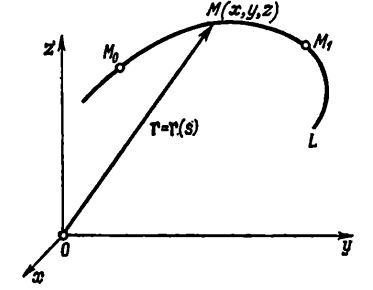
\includegraphics[width=0.5\textwidth]{comprimento-curva-parametro.jpg}
\caption{O raio vetor \(\alpha\) de um ponto \(M\) da curva \(L\)}
\label{fig:3-2-9}
\end{figure}


\subsection{A curvatura de uma Curva}

Se o vetor \(\alpha\) é dado pelas coordenadas
\begin{equation*}
	\alpha = x\,e_{1} + y\,e_{2} + z\, e_{3},
\end{equation*}
então
\begin{equation*}
	\tau = \dfrac{dx}{ds}\, e_{1} + \dfrac{dy}{ds}\, e_{2} + \dfrac{dz}{ds}\,e_{3}
\end{equation*}
e
\begin{equation*}
	\sqrt{\left(\dfrac{dx}{ds}\right)^{2}+\left(\dfrac{dy}{ds}\right)^{2}+\left(\dfrac{dz}{ds}\right)^{2}}=1.
\end{equation*}

Como \(\|\tau\| = 1\), o vetor \(d\tau/ds\) é \texttt{ortogonal} ao vetor \(\tau\).

O módulo do vetor \(d\tau/ds\) é
\begin{equation*}
	\left\|\dfrac{d\tau}{ds}\right\| = K.
\end{equation*}

Aqui, \(K\) é a curvatura da curva \(L\) no ponto \(M\).

A reta que tem a direção do vetor \(d\tau/ds\) e passa pelo ponto \(M\) da curva é denominada 
\texttt{normal principal} da curva no ponto \(M\).

Denotando o vetor unitário dessa direção por \(\boldsymbol{\nu}\), temos
\begin{equation}\label{eq:3-2-1}
	\dfrac{d\tau}{ds}= K\, \boldsymbol{\nu}.
\end{equation}

O inverso da curvatura de uma curva em um determinado ponto
é chamado de \texttt{raio de curvatura} da curva naquele ponto
e é denotado por \(R\),
\begin{equation*}
R=\dfrac{1}{K}.
\end{equation*}

Assim, a fórmula \eqref{eq:3-2-1} pode ser reescrita como
\begin{equation*}
\dfrac{d^{2}\alpha}{ds^{2}}=\dfrac{d\tau}{ds}=\dfrac{\boldsymbol{\nu}}{R}.
\end{equation*}

A partir disso,
\begin{equation*}
K=\dfrac{1}{R}=\left\|\dfrac{d^{2}\alpha}{ds^{2}}\right\|
\end{equation*}
ou
\begin{equation}\label{eq:3-2-2}
K=\dfrac{1}{R}=\sqrt{\left(\dfrac{d^{2}x}{ds^{2}}\right)^{2}+\left(\dfrac{d^{2}y}{ds^{2}}\right)^{2}+\left(\dfrac{d^{2}z}{ds^{2}}\right)^{2}}
\end{equation}

Usando a fórmula \eqref{eq:3-2-2}, podemos calcular a curvatura de uma curva em qualquer
ponto se a curva for especificada por equações paramétricas em
que o parâmetro é o comprimento do arco \(s\).

No caso particular de uma curva plana, um círculo de raio \(a\),
\begin{equation*}
\left\{
\begin{array}{cl}
x = & a \cos \dfrac{s}{a}\\[2ex]
y =& a \sen \dfrac{s}{a}
\end{array}
\right.
\end{equation*}
temos
\begin{equation*}
\dfrac{d^{2}x}{ds^{2}}=-\dfrac{1}{a}\cos\left(\dfrac{s}{a}\right), \quad
\dfrac{d^{2}y}{ds^{2}}=-\dfrac{1}{a}\sen \left(\dfrac{s}{a}\right)
\end{equation*}
e a fórmula \eqref{eq:3-2-2} produz
\begin{equation*}
K=\dfrac{1}{R}=\sqrt{\dfrac{1}{a^{2}}\cos^{2} \frac{s}{a}+ 
\dfrac{1}{a^{2}}\sen^{2} \frac{s}{a}}= \dfrac{1}{a}.
\end{equation*}

Isso significa que a curvatura de um círculo de raio \(a\) é constante e é igual ao inverso do 
raio do círculo.

Se a curva \(L\) for dada pela equação vetorial paramétrica \(\alpha=\alpha(t)\), onde o parâmetro \(t\) é arbitrário, então
\begin{equation}\label{eq:3-2-3}
K = \dfrac{1}{R}=\dfrac{\left\|\dfrac{d\alpha}{dt}\times \dfrac{d^{2}\alpha}{dt^{2}} \right\|}{\left\|\dfrac{d\alpha}{dt}\right\|^{3}}
\end{equation}

A fórmula \eqref{eq:3-2-3} permite calcular a curvatura da curva em qualquer ponto, desde que tenhamos uma especificação paramétrica arbitrária dessa curva.

\begin{exc}
Calcule a curvatura da curva helicoidal
\begin{equation*}
\alpha(t) = a\cos t\,e_{1} + a\sen t\, e_{2} + ht\, e_{3}.
\end{equation*}
\end{exc}

\solo Como a primeira e segunda derivada são dadas por,
\begin{align*}
\dfrac{d\alpha}{dt}&=  -a\sen t\,e_{1} + a\cos t\, e_{2} + h\, e_{3}.\\[2ex]
\dfrac{d^{2}\alpha}{dt^{2}}&= -a\cos t\,e_{1} - a\sen t\, e_{2} + 0\, e_{3}.
\end{align*}
e seu produto vetorial
\begin{equation*}
\dfrac{d\alpha}{dt}\times \dfrac{d^{2}\alpha}{dt^{2}}=
\begin{vmatrix}
e_{1} & e_{2} & e_{3}\\
-a\sen t& a\cos t & h\\
-a\cos t& -a\sen t & 0
\end{vmatrix}=ah\sen t\, e_{1}-ah\cos t\,e_{2}+a^{2}\,e_{3}.
\end{equation*}

Consequentemente,
\begin{equation*}
\left\|\dfrac{d\alpha}{dt}\times \dfrac{d^{2}\alpha}{dt^{2}}\right\|=a\sqrt{a^{2}+h^{2}} \quad \text{e}\quad 
\left\|\dfrac{d\alpha}{dt}\right\|= \sqrt{a^{2}+h^{2}}. 
\end{equation*}

Em virtude da fórmula \eqref{eq:3-2-3},
\begin{equation*}
K=\dfrac{1}{R}=\dfrac{a}{a^{2}+h^{2}}
\end{equation*}
ou
\begin{equation*}
R= \dfrac{a^{2}+h^{2}}{a}=\text{constante}.
\end{equation*}

Assim, uma curva helicoidal tem um raio de curvatura constante. \hfill \(\lozenge\)

%%%%
\section*{Exercícios Propostos}
%%%%
\begin{enumerate}[label=(\arabic*),ref=(\arabic*)]
\item Encontre o raio de curvatura de cada uma das curvas fornecidas.
\begin{enumerate}
\item \(\alpha =\ln \cos t\, e_{1} +\ln \sen t\, e_{2} +\sqrt{2t}\, e_{3}.\)
\item \(\alpha =t^{2}\,e_{1} + 2t^{3}\,e_{2}\)	
\item  \(\alpha =3t^{2}\, e_{1}+(3t-t^{3})\,e_{2}+2\, e_{3}\)\quad  para\quad  \(t=1\).
\item \(\alpha = a (\cos t + t \sen t)\,e_{1} + a (\sen t - t \cos t)\, e_{3}\)\quad  para \quad  \(t=\pi/2\).
\item \(\alpha =a \cosh t\, e_{1} +a\senh t\,e_{2} + at\,e_{3}\) \quad  em qualquer ponto \quad \(t\).
\end{enumerate}	
\end{enumerate}

